\documentclass[12pt,a4paper]{report}

% Limbă și diacritice
\usepackage{fontspec}
\defaultfontfeatures{Ligatures=TeX}
\setmainfont{Noto Serif}

% Margini & spațiere
\usepackage[margin=2.5cm]{geometry}
\usepackage{lmodern}
\linespread{1.1}

% Hiperlinkuri
\usepackage[hidelinks]{hyperref}

% Tabele & figuri
\usepackage{graphicx}
\usepackage{longtable}
\usepackage{float}
\usepackage{booktabs}
\usepackage{subcaption}
\usepackage{pgf-pie}
\usepackage[romanian]{babel}
\usepackage{array}

% Anexe
\usepackage[toc,page]{appendix}
\renewcommand{\appendixpagename}{Anexe}
\renewcommand{\appendixtocname}{Anexe}

% Matematică
\usepackage{amsmath, amssymb, amsthm}

% Enumerări
\usepackage{enumitem}

% Cod (Python)
\usepackage{minted}
\usemintedstyle{borland}

% Numerotări: Section -> I., Subsection -> 1.1 etc.
\renewcommand\thesection{\Roman{section}}
\setcounter{secnumdepth}{2}
\setcounter{tocdepth}{2}

% Informații titlu (modifică după nevoie)
\newcommand{\Universitate}{UNIVERSITATEA DE STAT DIN MOLDOVA}
\newcommand{\Facultate}{FACULTATEA DE MATEMATICĂ ȘI INFORMATICĂ}
\newcommand{\Departament}{DEPARTAMENTUL INFORMATICĂ}
\newcommand{\TitluProiect}{Analiza statistică a nivelului de activitate fizică zilnică (număr de pași)}
\newcommand{\Disciplina}{Statistica pentru Știința Datelor}
\newcommand{\Autor}{Ivan Majeru}
\newcommand{\Titular}{Conf. univ. dr. Ludmila Novac}
\newcommand{\An}{2025}

\begin{document}

% Pagina de titlu
\begin{titlepage}
  \centering
  {\Large \Universitate\par}
  {\large \Facultate\par}
  {\large \Departament\par}
  \vspace{2cm}
  {\LARGE Cercetare statistică\par}
  \vspace{0.5cm}
  {\Large \TitluProiect\par}
  \vspace{2.5cm}
  \begin{flushleft}
    \textbf{Autor:} \Autor\par
    \textbf{Titular disciplină:} \Titular\par
    \textbf{Disciplina:} \Disciplina\par
  \end{flushleft}
  \vfill
  {\An\par}
\end{titlepage}

\pagenumbering{roman}
\tableofcontents
\clearpage
\pagenumbering{arabic}

% INTRODUCERE
%\chapter*{Introducere}
%\addcontentsline{toc}{chapter}{Introducere}

% (De completat: contextul activității fizice, pașii/zi ca indicator,
% obiectivele proiectului și structura capitolelor.)

% I. OBSERVAȚIA STATISTICĂ
\section{Observația statistică}

\subsection{Scopul observației statistice}

Scopul prezentei cercetări statistice este de a analiza nivelul de activitate fizică zilnică, măsurat prin \texttt{Numar\_Pasi\_Zilnic} (numărul mediu de pași pe zi), în funcție de anumite caracteristici demografice și de stil de viață ale persoanelor adulte.

Mai exact, urmărim:
\begin{itemize}[leftmargin=1.2cm]
  \item descrierea distribuției numărului de pași pe zi în eșantionul studiat;
  \item compararea nivelului de activitate fizică între diferite categorii de persoane (după sex, tip de localitate, tip de ocupație, deținerea unui animal de companie);
  \item analiza relației dintre numărul de pași/zi și timpul liber dedicat activităților fizice (\texttt{Timp\_Liber\_Activ});
  \item construirea unor indicatori sintetici (medii, abateri, coeficienți de variație) pentru variabilele cantitative;
  \item ilustrarea, în mod aplicat, a metodelor studiate la disciplina \textit{Statistica pentru Știința Datelor}, folosind un set de date sintetice.
\end{itemize}

\subsection{Populația statistică}

\textbf{Populația statistică} vizată este formată din persoane adulte (cu vârsta între 18 și 70 de ani) care au reședința pe teritoriul Republicii Moldova și pentru care mersul pe jos reprezintă o componentă a activității zilnice (deplasări la locul de muncă, activități casnice, timp liber).

\textbf{Unitatea statistică} este \textit{individul} (persoana chestionată / simulată), pentru care se colectează atât informații demografice (sex, vârstă, tip de localitate), cât și informații privind stilul de viață (tip ocupație, timp liber activ, deținerea unui animal de companie) și nivelul de activitate fizică (numărul mediu de pași pe zi).

\subsection{Eșantionul statistic}

Pentru realizarea acestei cercetări s-a utilizat un \textbf{eșantion sintetic} de:
\[
n = 100 \text{ persoane.}
\]

Dimensiunea eșantionului a fost aleasă astfel încât:
\begin{itemize}[leftmargin=1.2cm]
  \item să fie suficient de mare pentru a permite aplicarea metodelor statistice (grupări, indicatori, serii dinamice);
  \item să rămână ușor de prezentat în tabele și anexe.
\end{itemize}

Datele nu provin dintr-un sondaj real, ci au fost generate în mod artificial (aleator) în Python, urmărind doar câteva \textit{proprietăți globale}:
\begin{itemize}
  \item vârste între 18 și 70 de ani;
  \item număr de pași/zi în intervalul 2000–20000;
  \item distribuție aproximativ echilibrată pe sexe;
  \item pondere mai mare a populației urbane față de cea rurală;
  \item prezența tuturor categoriilor de ocupație definite.
\end{itemize}

Este important de subliniat că:
\textbf{nu a fost impusă nicio legătură funcțională directă între variabile}
( de exemplu, \texttt{Numar\_Pasi\_Zilnic} nu a fost calculat în funcție de \texttt{Tip\_Ocupatie} sau \texttt{Timp\_Liber\_Activ} ). Toate variabilele au fost generate independent, folosind distribuții aleatoare simple (uniforme sau discrete), cu anumite probabilități presetate pentru categoriile calitative.

Prin urmare, eventualele corelații care vor apărea între variabile sunt \textbf{pur aleatorii}, iar interpretările rezultate trebuie privite ca exerciții metodologice, nu ca descrieri ale unui fenomen real.

\subsection{Metoda de observare}

Într-o cercetare reală, un astfel de studiu ar fi realizat prin:
\begin{itemize}[leftmargin=1.2cm]
  \item aplicarea unui chestionar (online sau față în față), pentru colectarea datelor demografice și de stil de viață;
  \item utilizarea aplicațiilor de monitorizare a pașilor de pe telefon sau ceas inteligent, pentru înregistrarea activității fizice zilnice.
\end{itemize}

În cadrul acestui proiect, pentru simplitate și pentru a pune accentul pe partea de analiză statistică, metoda de observare este \textbf{simulată} astfel:
\begin{itemize}
  \item toate variabilele sunt generate în Python, folosind funcții de generare aleatoare (\texttt{numpy.random}), cu reguli simple pentru intervale și probabilități;
  \item perioada de referință este \textit{conceptualizată} ca fiind o săptămână de monitorizare, dar în datele sintetice se lucrează direct cu valori de medie zilnică (\texttt{Numar\_Pasi\_Zilnic}) și ore pe săptămână (\texttt{Timp\_Liber\_Activ});
  \item nu se realizează o calibrare fină a distribuțiilor (de exemplu, nu se ajustează \texttt{Numar\_Pasi\_Zilnic} în funcție de vârstă sau ocupație).
\end{itemize}

Instrumentul principal de lucru este notebook-ul Jupyter, în care:
\begin{itemize}
  \item sunt generate datele brute;
  \item sunt efectuate prelucrările statistice (tabele, grupări, indicatori, grafice);
  \item sunt exportate tabelele și figurile utilizate în această lucrare.

\end{itemize}

\subsection{Caracteristicile statistice}

În cercetare sunt folosite următoarele variabile statistice:

\begin{itemize}[leftmargin=1.2cm]
  \item \texttt{ID} – identificator numeric unic pentru fiecare persoană (1, 2, \dots, 100). Este utilizat doar pentru referință și nu intră în analizele statistice propriu-zise.
  \item \texttt{Sex} – variabilă calitativă nominală cu două modalități: \textit{Masculin}, \textit{Feminin}. Este utilizată pentru a compara media numărului de pași zilnici între bărbați și femei.
  \item \texttt{Varsta} – vârsta persoanei, exprimată în ani împliniți. Este o variabilă cantitativă pe scală raport (se poate vorbi de zero absolut și de rapoarte semnificative: o persoană de 40 de ani este de două ori mai vârstnică decât una de 20 de ani).
  \item \texttt{Tip\_Localitate} – variabilă calitativă nominală cu două modalități: \textit{Urban}, \textit{Rural}. Permite studierea diferențelor de activitate fizică între mediul urban și mediul rural.
  \item \texttt{Numar\_Pasi\_Zilnic} – variabilă cantitativă pe scală raport, care reprezintă numărul mediu de pași efectuați zilnic de persoană. Este variabila principală analizată în proiect.
  \item \texttt{Tip\_Ocupatie} – variabilă calitativă nominală ce descrie tipul ocupației principale a persoanei. Categoriile considerate sunt:
  \begin{itemize}
    \item \textit{Sedentar};
    \item \textit{Moderat\_Activ};
    \item \textit{Activ};
    \item \textit{Student};
    \item \textit{Pensionar};
    \item \textit{Casnic/a}.
  \end{itemize}
  \item \texttt{Timp\_Liber\_Activ} – variabilă cantitativă pe scală raport, exprimată în ore pe săptămână, care indică timpul petrecut de persoană în activități fizice efective (sport, plimbări, alergare etc.) în afara obligațiilor profesionale.
  \item \texttt{Detine\_Animal\_Companie} – variabilă calitativă nominală, cu două modalități: \textit{Da} sau \textit{Nu}, indicând dacă persoana deține sau nu un animal de companie (de exemplu, câine, pisică).
\end{itemize}

Aceste variabile permit atât analize univariate (distribuții, indicatori), cât și analize bivariate (de exemplu, \texttt{Numar\_Pasi\_Zilnic} în funcție de \texttt{Sex} sau \texttt{Tip\_Ocupatie}).

2\subsection{Scale de măsurare}

În tabelul următor sunt sintetizate tipurile de variabile și scalele de măsurare utilizate:

\begin{table}[H]
\centering
\caption{Caracteristicile statistice și scalele de măsurare}
\label{tab:caracteristici_scale}
\begin{tabular}{lll}
\toprule
Variabilă & Tip & Scală de măsură \\
\midrule
\texttt{ID} & Calitativă (identificator) & Nominală \\
\texttt{Sex} & Calitativă & Nominală \\
\texttt{Varsta} & Cantitativă & Raport \\
\texttt{Tip\_Localitate} & Calitativă & Nominală \\
\texttt{Numar\_Pasi\_Zilnic} & Cantitativă & Raport \\
\texttt{Tip\_Ocupatie} & Calitativă & Nominală \\
\texttt{Timp\_Liber\_Activ} & Cantitativă & Raport \\
\texttt{Detine\_Animal\_Companie} & Calitativă & Nominală \\
\bottomrule
\end{tabular}
\end{table}

Faptul că principalele variabile cantitative sunt pe scală raport permite calcularea tuturor indicatorilor de tendință centrală și de variație (media aritmetică, mediana, modul, varianța, abaterea standard, coeficientul de variație), precum și analizarea unor serii dinamice.

\subsection{Sursa datelor și procedura de generare a datelor sintetice}

Datele utilizate în această cercetare sunt \textbf{date primare sintetice}, generate integral în Python, într-un notebook Jupyter. Nu s-a aplicat un chestionar real, iar valorile nu corespund unor persoane concrete.

Procedura simplificată de generare a fost următoarea:

\begin{enumerate}[leftmargin=1.2cm,label=\arabic*.]
  \item \textbf{Stabilirea variabilelor și a dimensiunii eșantionului}\\
  S-a fixat numărul de observații la $n = 100$ și s-a definit schema de variabile: \texttt{ID}, \texttt{Sex}, \texttt{Varsta}, \texttt{Tip\_Localitate}, \texttt{Numar\_Pasi\_Zilnic}, \texttt{Tip\_Ocupatie}, \texttt{Timp\_Liber\_Activ}, \texttt{Detine\_Animal\_Companie}.

  \item \textbf{Generarea variabilei \texttt{Varsta}}\\
  Pentru fiecare observație, vârsta a fost generată ca număr întreg în intervalul:
  \[
  18 \leq \texttt{Varsta} \leq 70,
  \]
  folosind o distribuție uniformă (toate vârstele din interval având aceeași probabilitate de apariție).

  \item \textbf{Generarea variabilelor calitative \texttt{Sex} și \texttt{Tip\_Localitate}}\\
  \texttt{Sex} a fost generat ca variabilă binară (\textit{Masculin}/\textit{Feminin}), de obicei cu probabilități aproximativ egale (în jur de 0{,}5 pentru fiecare categorie), astfel încât eșantionul să fie aproape echilibrat.\\[0.2cm]
  \texttt{Tip\_Localitate} a fost generat cu două valori posibile, \textit{Urban} și \textit{Rural}, cu o probabilitate mai mare pentru mediul urban (de exemplu, \textasciitilde 65\% Urban, \textasciitilde 35\% Rural), reflectând urbanizarea mai accentuată.

  \item \textbf{Generarea variabilelor \texttt{Tip\_Ocupatie} și \texttt{Detine\_Animal\_Companie}}\\
  \texttt{Tip\_Ocupatie} a fost generat aleator, atribuind fiecărei persoane una dintre categoriile:
  \textit{Sedentar}, \textit{Moderat\_Activ}, \textit{Activ}, \textit{Student}, \textit{Pensionar}, \textit{Casnic/a}. Probabilitățile au fost alese astfel încât toate categoriile să fie reprezentate, fără însă a modela explicit structura reală a populației.\\[0.2cm]
  \texttt{Detine\_Animal\_Companie} a fost generat ca variabilă binară (\textit{Da}/\textit{Nu}), prin selecție aleatoare, cu o pondere moderată a proprietarilor de animale de companie.

  \item \textbf{Generarea timpului liber activ}\\
  \texttt{Timp\_Liber\_Activ} a fost generat ca număr întreg de ore pe săptămână, în interiorul unui interval prestabilit (de exemplu, 0–15 ore/săptămână), utilizând o generare aleatoare simplă. Nu s-a impus o relație directă între \texttt{Timp\_Liber\_Activ} și alte variabile (de exemplu, ocupatia sau vârsta).

  \item \textbf{Generarea numărului de pași pe zi}\\
  Variabila principală \texttt{Numar\_Pasi\_Zilnic} a fost generată ca număr întreg în intervalul:
  \[
  2000 \leq \texttt{Numar\_Pasi\_Zilnic} \leq 20000,
  \]
  folosind o distribuție uniformă. Aceasta înseamnă că orice valoare între 2000 și 20000 de pași/zi este, în principiu, la fel de probabilă ca oricare alta, în cadrul simulării.

  % Important:
  Nu s-a introdus \textbf{nicio ajustare suplimentară} care să lege \texttt{Numar\_Pasi\_Zilnic} de \texttt{Tip\_Ocupatie}, \texttt{Timp\_Liber\_Activ}, \texttt{Varsta} sau \texttt{Detine\_Animal\_Companie}. Toate aceste variabile au fost generate independent, astfel încât structura datelor reflectă strict aleatorul, nu un model realist al comportamentului uman.

  \item \textbf{Curățarea minimă și stocarea datelor}\\
  După generare, s-a verificat doar că toate valorile respectă domeniile stabilite (de exemplu, nici o vârstă în afara intervalului 18–70, niciun număr de pași în afara intervalului 2000–20000, nici o categorie în afara setului definit). Setul de date rezultat a fost stocat într-un obiect \texttt{DataFrame} (\texttt{pandas}) și salvat pentru a fi utilizat ulterior în analize și pentru exportul tabelelor în LaTeX.
\end{enumerate}

În concluzie, sursa datelor este un \textbf{notebook Jupyter} în care datele au fost generate complet aleator, cu respectarea doar a unor limite de interval și a unei structuri de categorii. Interpretările obținute în capitolele următoare au rolul de a ilustra tehnicile statistice, nu de a descrie un fenomen real măsurat în teren.

% II. SISTEMATIZAREA ȘI PREZENTAREA DATELOR
\section{Sistematizarea și prezentarea datelor}

\subsection{Prezentarea bazei de date}
% Aici vei pune un tabel cu primele 5-10 înregistrări
% exportat din Jupyter (ex: cu to_latex()).

Baza de date utilizată în acest proiect conține informații despre nivelul de activitate fizică zilnică, măsurat prin numărul mediu de pași pe zi, precum și despre câteva caracteristici demografice și de stil de viață ale persoanelor investigate.

Setul de date este constituit din \(n = 100\) observații (persoane), fiecare observație fiind identificată printr-un \textit{ID} unic. Pentru fiecare persoană sunt înregistrate următoarele variabile:

\begin{itemize}
    \item \textbf{ID} -- identificator numeric unic al persoanei (scală nominală).
    \item \textbf{Sex} -- sexul persoanei, cu două modalități: \textit{Masculin}, \textit{Feminin} (scală nominală).
    \item \textbf{Vârstă (\textit{Varsta})} -- vârsta în ani împliniți (scală de raport).
    \item \textbf{Tip localitate (\textit{Tip\_Localitate})} -- mediul de rezidență: \textit{Urban}, \textit{Rural} (scală nominală).
    \item \textbf{Număr pași zilnic (\textit{Numar\_Pasi\_Zilnic})} -- numărul mediu de pași pe zi (scală de raport); aceasta este variabila principală analizată în proiect.
    \item \textbf{Tip ocupație (\textit{Tip\_Ocupatie})} -- categoria ocupațională a persoanei: \textit{Sedentar}, \textit{Moderat\_Activ}, \textit{Activ}, \textit{Student}, \textit{Pensionar}, \textit{Casnic/a} (scală nominală).
    \item \textbf{Timp liber activ (\textit{Timp\_Liber\_Activ})} -- numărul de ore pe săptămână dedicate activităților fizice în timpul liber (scală de raport).
\end{itemize}

Pentru variabilele cantitative principale (\textit{Varsta}, \textit{Numar\_Pasi\_Zilnic}, \textit{Timp\_Liber\_Activ}) se poate observa, pe baza indicatorilor descriptivi calculați în Python, că:

\begin{itemize}
    \item vârsta persoanelor din eșantion variază între \(18\) și \(70\) de ani, cu o valoare medie de aproximativ \(39{,}6\) ani;
    \item numărul mediu de pași zilnic este cuprins între aproximativ \(1500\) și \(12832\) de pași, cu o medie de circa \(7551\) pași/zi;
    \item timpul liber activ variază între \(0\) și aproximativ \(11{,}7\) ore pe săptămână, cu o medie de aproximativ \(2{,}24\) ore/săptămână.
\end{itemize}

În \autoref{tab:head-baza-date} este prezentat un extras din baza de date, cu primele 10 înregistrări, pentru a ilustra structura concretă a datelor analizate.

\begin{table}[h!]
    \centering
    \caption{Primele 10 înregistrări din baza de date}
    \label{tab:head-baza-date}
    \begin{tabular}{r l r l r l r}
        \hline
        ID & Sex & Varsta & Tip\_Localitate & Numar\_Pasi\_Zilnic & Tip\_Ocupatie \\
        \hline
         1 & Masculin & 41 & Rural & 10667 & Sedentar      \\
         2 & Feminin  & 35 & Urban &  5730 & Moderat\_Activ\\
         3 & Feminin  & 41 & Urban &  8609 & Sedentar      \\
         4 & Feminin  & 18 & Urban &  9436 & Sedentar      \\
         5 & Masculin & 36 & Urban &  5182 & Sedentar      \\
         6 & Masculin & 45 & Rural &  7351 & Activ         \\
         7 & Masculin & 62 & Urban &  1500 & Student       \\
         8 & Feminin  & 32 & Urban &  4939 & Activ         \\
         9 & Feminin  & 27 & Rural &  6868 & Casnic/a      \\
        10 & Feminin  & 32 & Urban &  4380 & Moderat\_Activ\\
        \hline
    \end{tabular}
\end{table}

\pagebreak

\subsection{Distribuția după variabile calitative}
% Tabele frecvențe + grafice (bar/pie)

\subsubsection{Distribuția după sex}
% Tabelul de frecvențe absolute/relative (de completat)

Pentru a analiza structura eșantionului din punct de vedere al sexului, s-a întocmit tabelul de frecvențe absolute și relative prezentat în \autoref{tab:freq-sex}.

\begin{table}[h!]
    \centering
    \caption{Distribuția eșantionului după sex}
    \label{tab:freq-sex}
    \begin{tabular}{l r r}
        \hline
        \textbf{Sex} & \textbf{Frecvență} & \textbf{Pondere (\%)} \\
        \hline
        Feminin  & 47 & 47{,}0 \\
        Masculin & 53 & 53{,}0 \\
        \hline
        \textbf{Total} & \textbf{100} & \textbf{100{,}0} \\
        \hline
    \end{tabular}
\end{table}

Reprezentarea grafică a acestei distribuții este prezentată în \autoref{fig:sex-pie}.

\begin{figure}[h!]
    \centering
    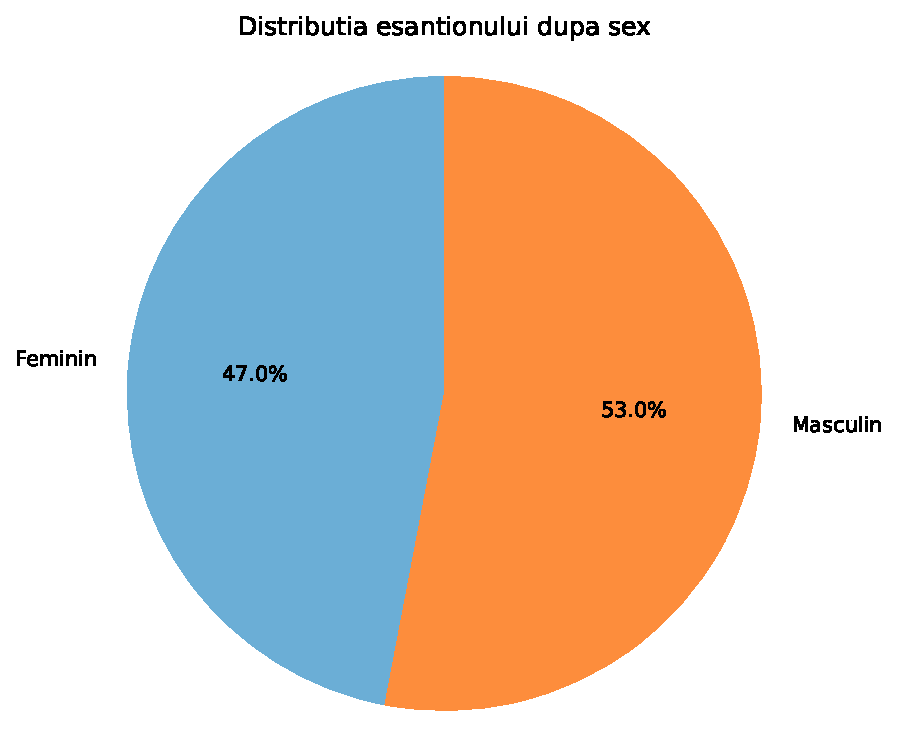
\includegraphics[width=0.4\textwidth]{../figuri/sex_distribution.pdf}
    \caption{Distribuția eșantionului după sex}
    \label{fig:sex-pie}
\end{figure}

% \begin{figure}[h!]
%     \centering
%     \begin{tikzpicture}
%         \pie[
%             text=legend,
%             radius=2,
%             color={blue!50, orange!70}
%         ]{
%             47/Feminin,
%             53/Masculin
%         }
%     \end{tikzpicture}
%     \caption{Distribuția eșantionului după sex}
%     \label{fig:sex-pie}
% \end{figure}

\subsubsection{Distribuția după tip localitate}
% tabel + grafic
Pentru a analiza structura eșantionului din punct de vedere al localitatii, s-a întocmit tabelul de frecvențe absolute și relative prezentat în \autoref{tab:freq-local}.

\begin{table}[h!]
    \centering
    \caption{Distribuția eșantionului după localitate}
    \label{tab:freq-local}
    \begin{tabular}{l r r}
        \hline
        \textbf{Tip Localitate} & \textbf{Frecvență} & \textbf{Pondere (\%)} \\
        \hline
        Rural  & 43 & 43{,}0 \\
        Urban & 57 & 57{,}0 \\
        \hline
        \textbf{Total} & \textbf{100} & \textbf{100{,}0} \\
        \hline
    \end{tabular}
\end{table}

Reprezentarea grafică a acestei distribuții este prezentată în \autoref{fig:loc-pie}.

\begin{figure}[h!]
    \centering
    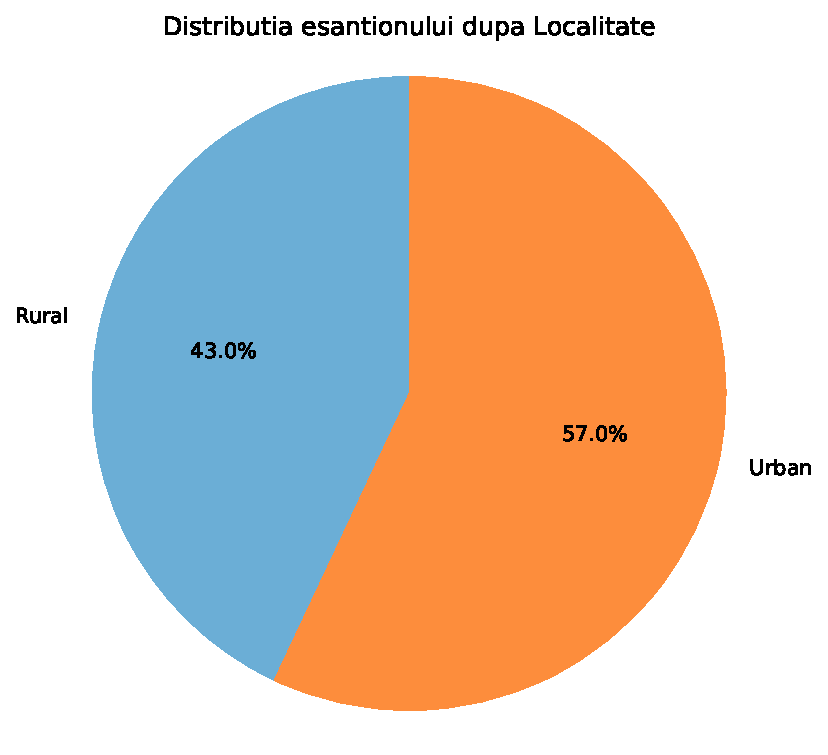
\includegraphics[width=0.4\textwidth]{../figuri/localitate_distr.pdf}
    \caption{Distribuția eșantionului după Localitate}
    \label{fig:loc-pie}
\end{figure}

\subsubsection{Distribuția după tip ocupație}
% tabel cu frecvențe + grafic bar ordonat descrescător
Pentru a analiza structura eșantionului din punct de vedere al tipului de ocupatie, s-a întocmit tabelul de frecvențe absolute și relative prezentat în \autoref{tab:freq-ocupatie}.

\begin{table}[h!]
    \centering
    \caption{Distribuția eșantionului după tipul de ocupație}
    \label{tab:freq-ocupatie}
    \begin{tabular}{l r r}
        \hline
        \textbf{Tip ocupație} & \textbf{Frecvență absolută} & \textbf{Frecvență relativă (\%)} \\
        \hline
        Activ          & 25 & 25{,}0 \\
        Casnic/a       & 13 & 13{,}0 \\
        Moderat Activ  & 19 & 19{,}0 \\
        Pensionar      & 12 & 12{,}0 \\
        Sedentar       & 20 & 20{,}0 \\
        Student        & 11 & 11{,}0 \\
        \hline
        \textbf{Total} & \textbf{100} & \textbf{100{,}0} \\
        \hline
    \end{tabular}
\end{table}

Reprezentarea grafică a acestei distribuții este prezentată în \autoref{fig:ocupatie-pie}.

\begin{figure}[h!]
    \centering
    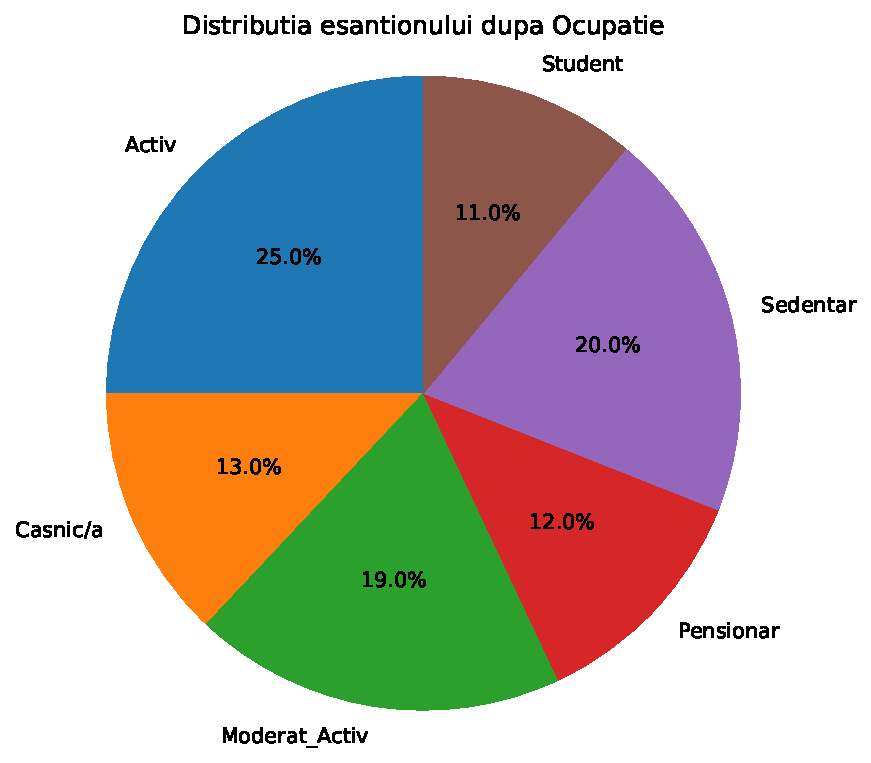
\includegraphics[width=0.6\textwidth]{../figuri/ocupatie_distr.pdf}
    \caption{Distribuția eșantionului după Localitate}
    \label{fig:loc-pie}
\end{figure}

\pagebreak

\subsection{Distribuții pentru variabilele cantitative}

\subsubsection{Distribuția vârstei}
% Tabel cu intervale, frecvențe, frecvențe relative, cumulative.
% Histogramă exportată din Jupyter.

Pentru a analiza distribuția vârstei persoanelor din eșantion, am construit o serie de repartiție pe clase de vârstă. Intervalele de vârstă au fost definite în categorii interpretabile, iar frecvențele absolute și relative corespunzătoare sunt prezentate în Tabelul~\ref{tab:dist-varsta}.

\begin{table}[h!]
    \centering
    \caption{Distribuția eșantionului după clase de vârstă}
    \label{tab:dist-varsta}
    \begin{tabular}{l r r}
        \hline
        \textbf{Clasă de vârstă (ani)} & \textbf{Frecvență} & \textbf{Pondere (\%)} \\
        \hline
        {[}18, 25)                      & 13 & 13{,}0 \\
        {[}25, 35)                      & 22 & 22{,}0 \\
        {[}35, 45)                      & 33 & 33{,}0 \\
        {[}45, 55)                      & 21 & 21{,}0 \\
        {[}55, 65)                       & 6 &  6{,}0 \\
        {[}65, 75)                       & 5 &  5{,}0 \\
        \hline
        \textbf{Total}                 & \textbf{100} & \textbf{100{,}0} \\
        \hline
    \end{tabular}
\end{table}

Distribuția grafică a vârstei este ilustrată în histograma din Figura~\ref{fig:varsta-hist}. Se observă o concentrare a majorității respondenților în categoriile de vârstă medie, în special între 35 și 45 de ani, care reprezintă cea mai mare pondere (\(33\%\)). Pe măsură ce vârsta crește, frecvența scade, indicând o proporție mai mică de persoane vârstnice în eșantion.

\begin{figure}[h!]
    \centering
    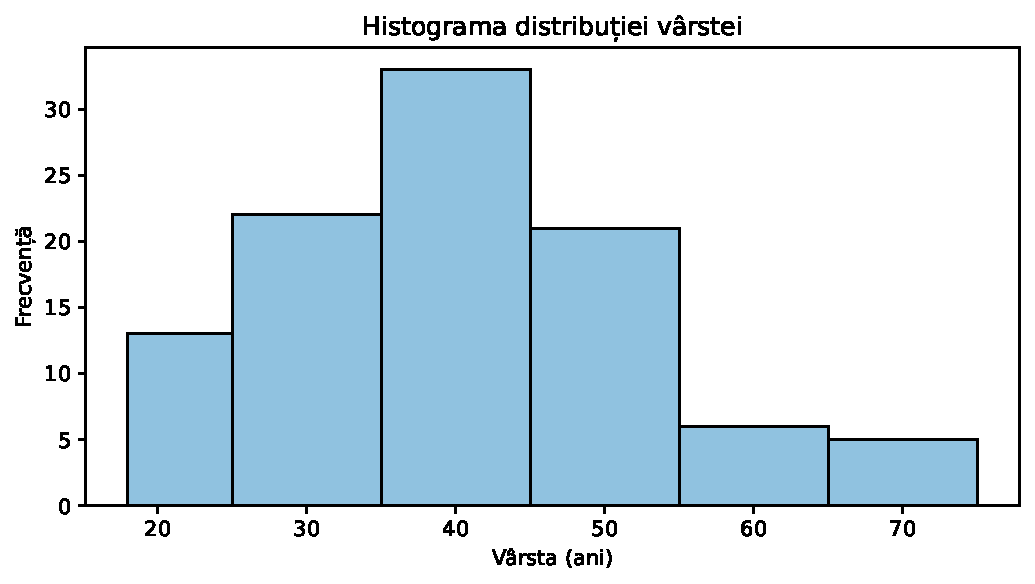
\includegraphics[width=0.7\textwidth]{../figuri/varsta_hist.pdf}
    \caption{Histograma distribuției vârstei}
    \label{fig:varsta-hist}
\end{figure}

Complementar, boxplot-ul din Figura~\ref{fig:varsta-box} evidențiază valorile medianei, ale quartilelor și eventualele valori extreme ale variabilei \textit{Varsta}.

\begin{figure}[h!]
    \centering
    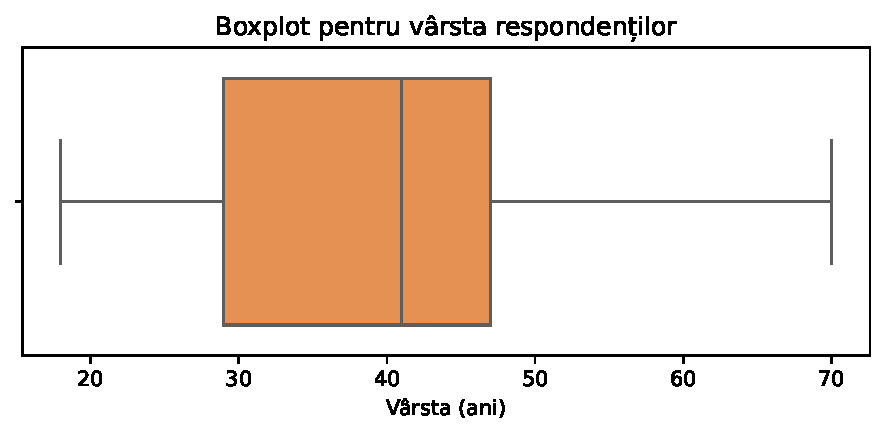
\includegraphics[width=0.7\textwidth]{../figuri/varsta_boxplot.pdf}
    \caption{Boxplot pentru vârsta respondenților}
    \label{fig:varsta-box}
\end{figure}

\subsubsection{Distribuția numărului de pași/zi}
% Definirea intervalelor, tabel, histogramă, eventual categorii de activitate.

Pentru a analiza distribuția variabilei principale \textit{Numar\_Pasi\_Zilnic}, am construit o serie de repartiție pe clase. Numărul de clase (intervale) a fost determinat folosind \textbf{regula lui Sturges}, care este o metodă euristică frecvent utilizată în statistică pentru alegerea numărului optim de intervale într-o histogramă.

Regula lui Sturges este definită prin formula:
\begin{equation}
    k = 1 + \lceil \log_2 n \rceil
\end{equation}
unde \(k\) reprezintă numărul de clase, iar \(n\) este numărul de observații din eșantion. În cazul nostru, cu \(n = 100\) observații, obținem:
\begin{equation}
    k = 1 + \lceil \log_2 100 \rceil = 1 + \lceil 6{,}64 \rceil = 1 + 7 = 8 \text{ clase}
\end{equation}

Pe baza acestui calcul, am împărțit intervalul valorilor numărului de pași zilnic (de la 1500 la aproximativ 12800 de pași) în 8 clase de amplitudine aproximativ egală. Intervalele au fost rotunjite pentru a facilita interpretarea. Distribuția frecvențelor absolute și relative pe aceste clase este prezentată în Tabelul~\ref{tab:dist-pasi}.

\begin{table}[h!]
    \centering
    \caption{Distribuția eșantionului după numărul de pași zilnic}
    \label{tab:dist-pasi}
    \begin{tabular}{l r r}
        \hline
        \textbf{Clasă (nr. pași/zi)} & \textbf{Frecvență absolută} & \textbf{Frecvență relativă (\%)} \\
        \hline
        {[}1500, 2900)   &  2 &  2{,}0 \\
        {[}2900, 4300)   &  4 &  4{,}0 \\
        {[}4300, 5700)   & 13 & 13{,}0 \\
        {[}5700, 7200)   & 26 & 26{,}0 \\
        {[}7200, 8600)   & 22 & 22{,}0 \\
        {[}8600, 10000)  & 21 & 21{,}0 \\
        {[}10000, 11400) &  8 &  8{,}0 \\
        {[}11400, 12800) &  3 &  3{,}0 \\
        \hline
        \textbf{Total}   & \textbf{100} & \textbf{100{,}0} \\
        \hline
    \end{tabular}
\end{table}

Reprezentarea grafică a distribuției este prezentată în histograma din Figura~\ref{fig:pasi-hist}. Se observă că distribuția numărului de pași zilnic prezintă o formă aproximativ simetrică, cu o concentrare a valorilor în jurul intervalului central {[}5700, 7200), care conține cea mai mare pondere de observații (\(26\%\)). Valorile extreme (sub 4300 de pași sau peste 10000 de pași) sunt mai puțin frecvente, ceea ce sugerează că majoritatea persoanelor din eșantion au un nivel moderat de activitate fizică zilnică.

\begin{figure}[h!]
    \centering
    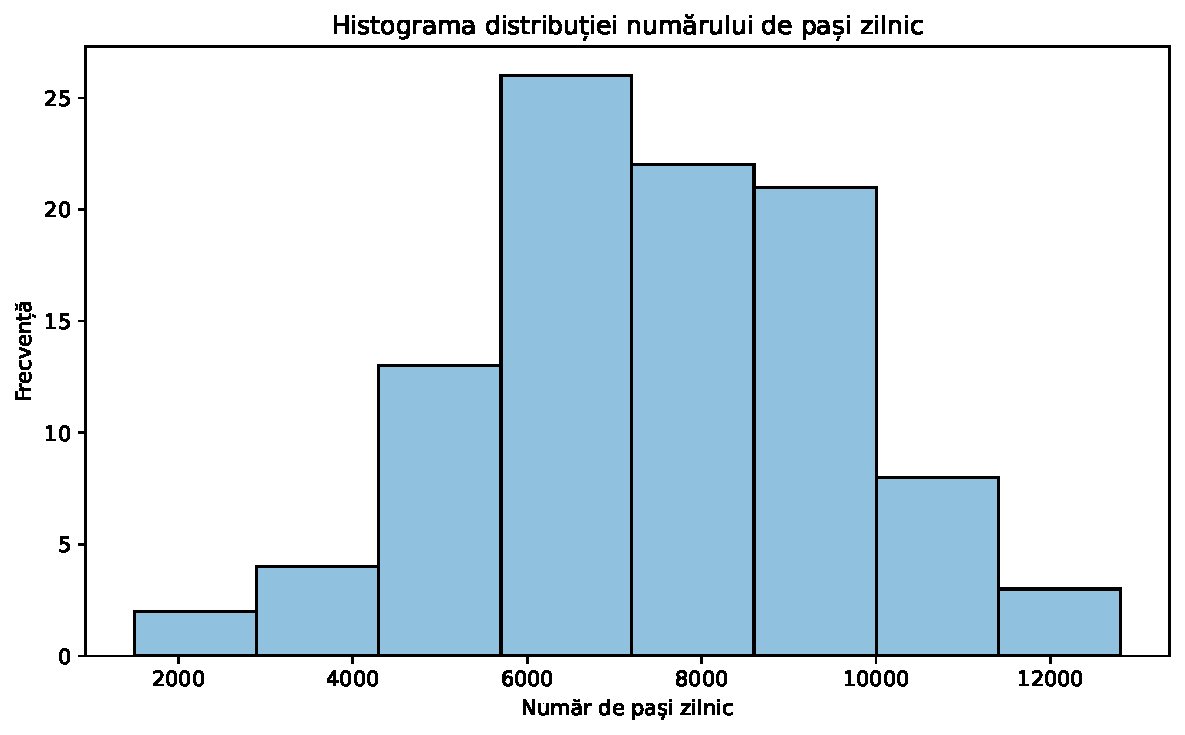
\includegraphics[width=0.75\textwidth]{../figuri/pasi_hist.pdf}
    \caption{Histograma distribuției numărului de pași zilnic}
    \label{fig:pasi-hist}
\end{figure}

Complementar, boxplot-ul din Figura~\ref{fig:pasi-box} oferă o vizualizare sintetică a caracteristicilor distribuției, evidențiind mediana, quartilele și eventualele valori extreme (outliers) ale variabilei \textit{Numar\_Pasi\_Zilnic}.

\begin{figure}[h!]
    \centering
    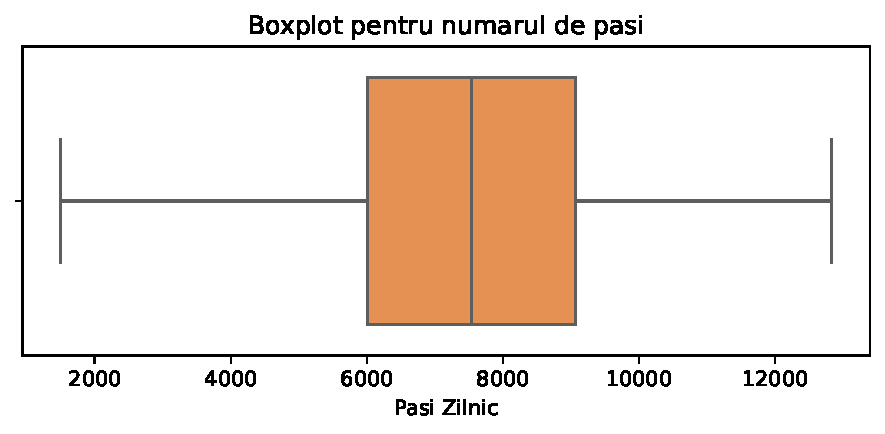
\includegraphics[width=0.7\textwidth]{../figuri/pasi_boxplot.pdf}
    \caption{Boxplot pentru numărul de pași zilnic}
    \label{fig:pasi-box}
\end{figure}

\subsection{Analiză bivariată descriptivă}

\subsubsection{Număr mediu de pași pe zi după sex}
% Tabel: Sex vs. media, mediana, abaterea standard.
% Bar chart cu media pașilor.

Pentru a investiga dacă există diferențe în nivelul de activitate fizică zilnică între bărbați și femei, am analizat distribuția variabilei \textit{Numar\_Pasi\_Zilnic} pe grupe de \textit{Sex}. În Tabelul~\ref{tab:pasi-sex} sunt prezentați, pentru fiecare categorie de sex, numărul de observații, media, mediana și deviația standard a numărului de pași zilnic.

\begin{table}[h!]
    \centering
    \caption{Indicatori descriptivi ai numărului de pași zilnic după sex}
    \label{tab:pasi-sex}
    \begin{tabular}{l r r r r}
        \hline
        \textbf{Sex} & \textbf{Frecvență} & \textbf{Medie} & \textbf{Mediana} & \textbf{Deviație standard} \\
        \hline
        Feminin  & 47 & 7448{,}11 & 7120{,}0 & 2078{,}25 \\
        Masculin & 53 & 7641{,}58 & 7783{,}0 & 2284{,}09 \\
        \hline
    \end{tabular}
\end{table}

Se observă că bărbații au, în medie, un număr ușor mai mare de pași zilnic (\(7641{,}58\) pași) comparativ cu femeile (\(7448{,}11\) pași). De asemenea, mediana este mai ridicată pentru bărbați (\(7783\) pași) decât pentru femei (\(7120\) pași), ceea ce sugerează că, în general, bărbații tind să aibă un nivel de activitate fizică zilnică ceva mai ridicat. Deviațiile standard sunt relativ apropiate (aproximativ \(2078\) pași pentru femei și \(2284\) pași pentru bărbați), indicând o variabilitate comparabilă a numărului de pași în cadrul fiecărui grup.

Distribuția numărului de pași zilnic în funcție de sex este ilustrată prin boxplot-ul din Figura~\ref{fig:pasi-sex-box}, care permite compararea poziției centrale și a gradului de dispersie pentru cele două categorii de sex, precum și identificarea eventualelor valori extreme.

\begin{figure}[h!]
    \centering
    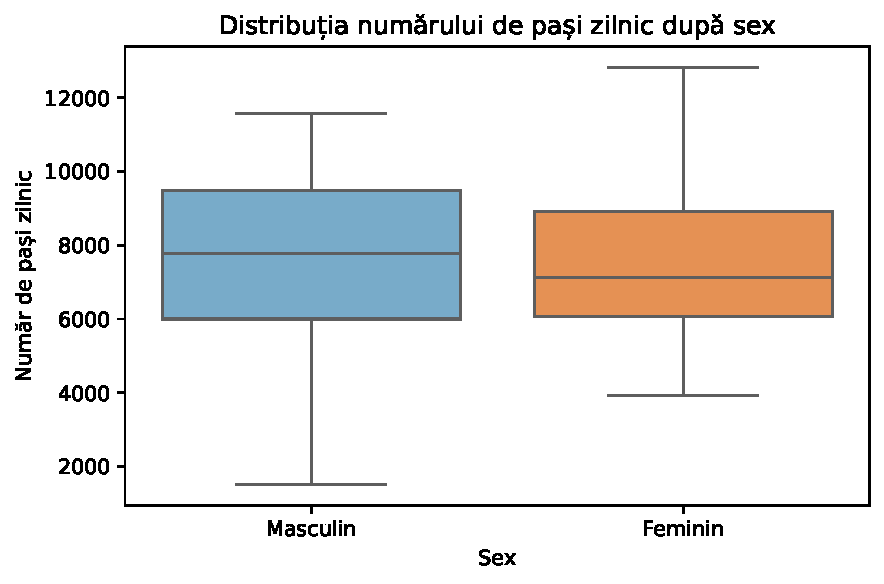
\includegraphics[width=0.6\textwidth]{../figuri/pasi_sex_boxplot.pdf}
    \caption{Distribuția numărului de pași zilnic după sex (boxplot)}
    \label{fig:pasi-sex-box}
\end{figure}

\pagebreak

Pentru a examina mai detaliat forma distribuției în cadrul fiecărui grup, în Figura~\ref{fig:pasi-sex-hist} sunt prezentate histograme suprapuse ale numărului de pași zilnic pentru bărbați și femei. Se poate observa că distribuțiile celor două grupe sunt relativ asemănătoare ca formă, cu o concentrare a valorilor în intervalele medii de pași zilnic, diferențele dintre sexe fiind mai degrabă de nivel (poziție centrală) decât de formă sau dispersie.

\begin{figure}[h!]
    \centering
    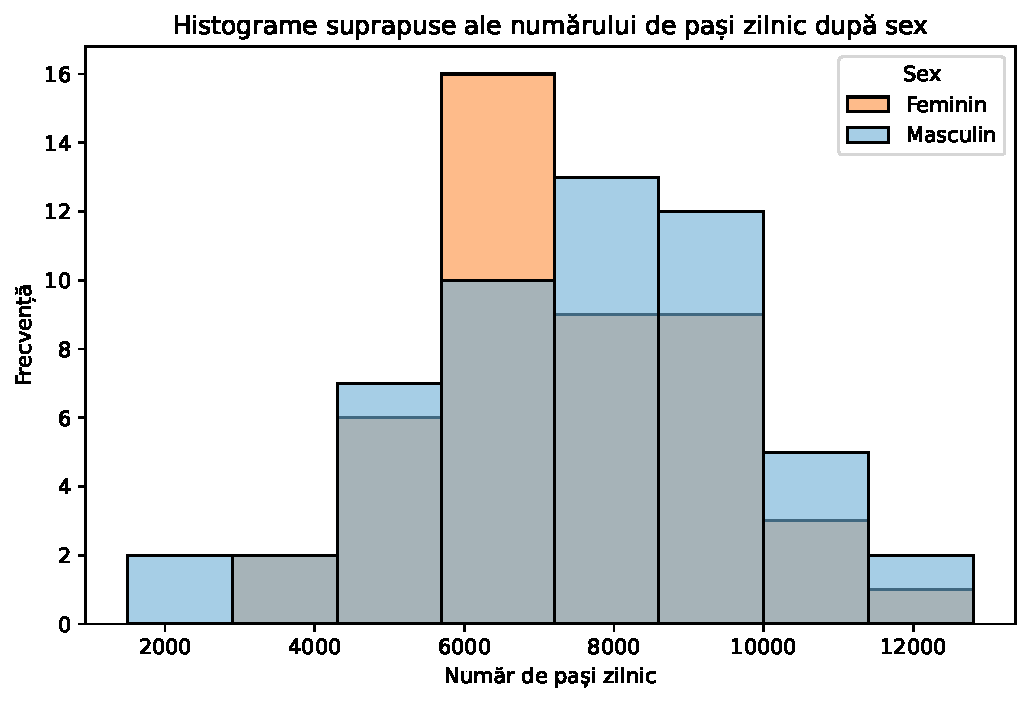
\includegraphics[width=0.75\textwidth]{../figuri/pasi_sex_hist_overlay.pdf}
    \caption{Histograme suprapuse ale numărului de pași zilnic după sex}
    \label{fig:pasi-sex-hist}
\end{figure}

\pagebreak

În plus, Figura~\ref{fig:pasi-sex-bar} prezintă o comparație directă a mediilor numărului de pași zilnic pentru cele două categorii de sex, împreună cu bare de eroare reprezentând deviația standard. Această reprezentare subliniază diferența relativ mică între mediile celor două grupe, precum și variabilitatea comparabilă în cadrul fiecărui grup.

\begin{figure}[h!]
    \centering
    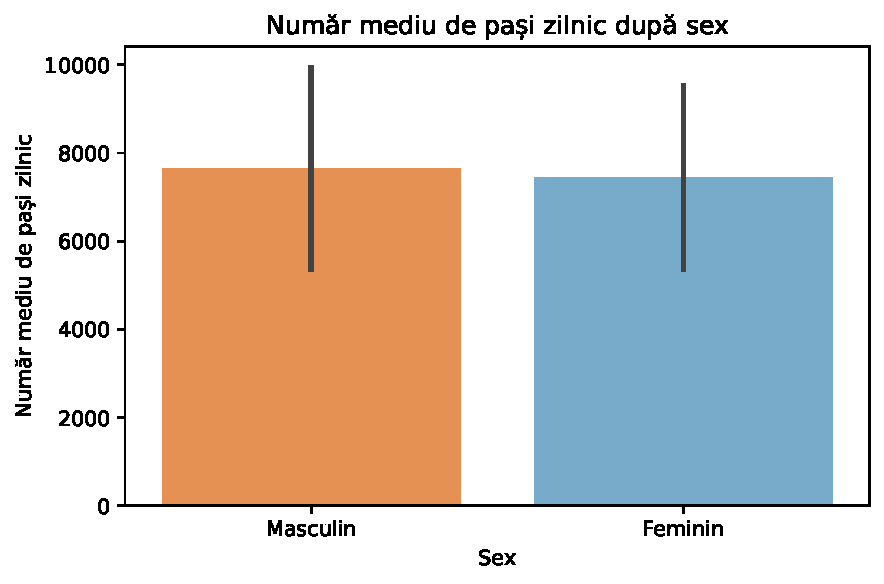
\includegraphics[width=0.6\textwidth]{../figuri/pasi_sex_barplot.pdf}
    \caption{Număr mediu de pași zilnic după sex cu bare de eroare (deviație standard)}
    \label{fig:pasi-sex-bar}
\end{figure}


\subsubsection{Număr mediu de pași pe zi după tip localitate}
% Urban vs. rural.

Pentru a analiza dacă mediul de rezidență influențează nivelul de activitate fizică zilnică, am comparat valorile variabilei \textit{Numar\_Pasi\_Zilnic} între persoanele din mediul urban și cele din mediul rural. În Tabelul~\ref{tab:pasi-localitate} sunt prezentați, pentru fiecare tip de localitate, numărul de observații, media, mediana și deviația standard a numărului de pași zilnic.

\begin{table}[h!]
    \centering
    \caption{Indicatori descriptivi ai numărului de pași zilnic după tipul localității}
    \label{tab:pasi-localitate}
    \begin{tabular}{l r r r r}
        \hline
        \textbf{Tip localitate} & \textbf{Frecvență} & \textbf{Medie} & \textbf{Mediana} & \textbf{Deviație standard} \\
        \hline
        Rural & 43 & 7622{,}72 & 7525{,}0 & 2106{,}38 \\
        Urban & 57 & 7496{,}28 & 7552{,}0 & 2252{,}62 \\
        \hline
    \end{tabular}
\end{table}

Se observă că diferențele între mediul urban și rural sunt relativ mici. Persoanele din mediul rural au, în medie, un număr ușor mai mare de pași zilnic (\(7622{,}72\) pași) comparativ cu cele din mediul urban (\(7496{,}28\) pași), diferența fiind de aproximativ \(126\) pași pe zi. Medianele sunt foarte apropiate (\(7525\) pași pentru rural și \(7552\) pași pentru urban), ceea ce sugerează că distribuțiile celor două grupe sunt similare ca poziție centrală. Deviațiile standard sunt, de asemenea, comparabile (aproximativ \(2106\) pași pentru rural și \(2253\) pași pentru urban), indicând o variabilitate similară în cadrul fiecărui grup.

Distribuția numărului de pași zilnic în funcție de tipul localității este ilustrată prin boxplot-ul din Figura~\ref{fig:pasi-localitate-box}, care permite compararea poziției centrale și a dispersiei pentru cele două grupe.

\begin{figure}[h!]
    \centering
    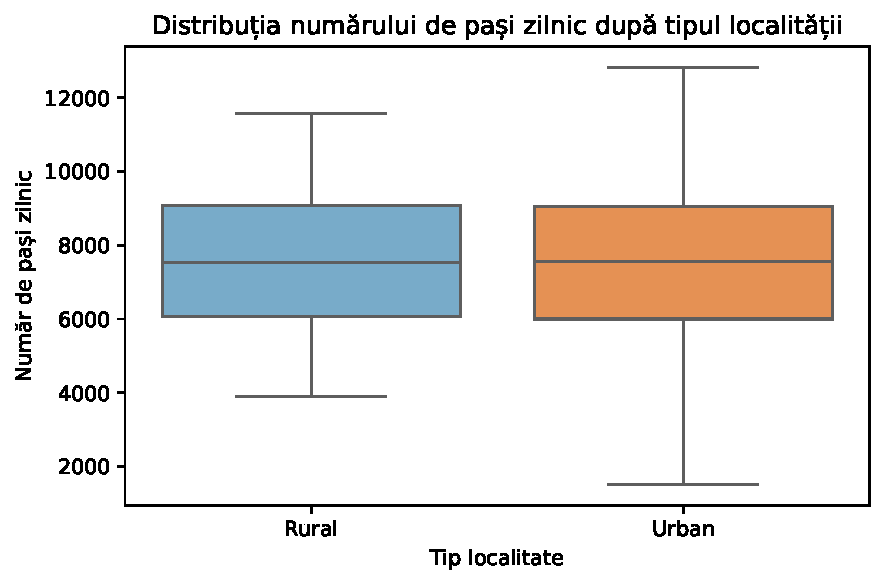
\includegraphics[width=0.6\textwidth]{../figuri/pasi_localitate_boxplot.pdf}
    \caption{Distribuția numărului de pași zilnic după tipul localității (boxplot)}
    \label{fig:pasi-localitate-box}
\end{figure}

În plus, Figura~\ref{fig:pasi-localitate-bar} prezintă comparația directă a mediilor numărului de pași zilnic pentru mediul urban și rural, împreună cu bare de eroare reprezentând deviația standard. Această reprezentare subliniază faptul că diferența între cele două medii este minimă, iar intervalele de variabilitate se suprapun în mare măsură.

\begin{figure}[h!]
    \centering
    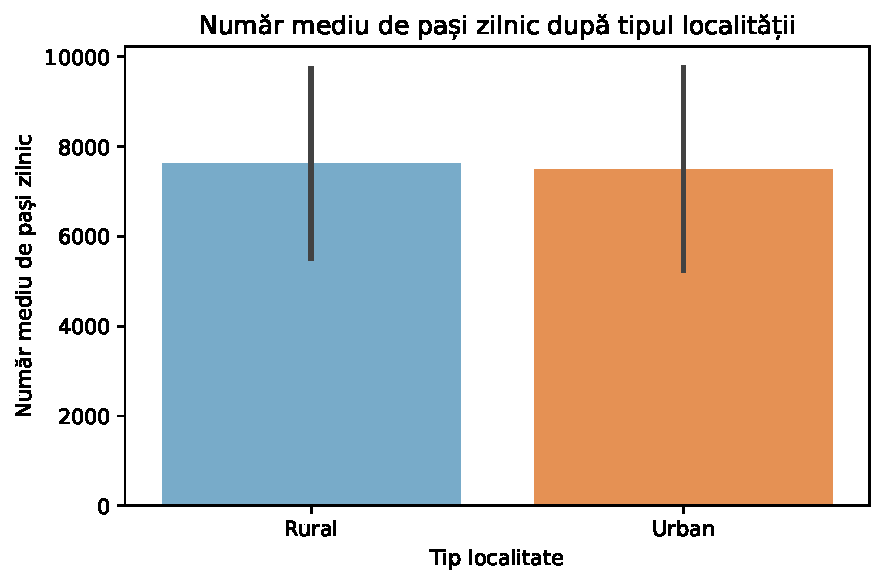
\includegraphics[width=0.6\textwidth]{../figuri/pasi_localitate_barplot.pdf}
    \caption{Număr mediu de pași zilnic după tipul localității cu bare de eroare (deviație standard)}
    \label{fig:pasi-localitate-bar}
\end{figure}

\subsubsection{Număr mediu de pași pe zi după tip ocupație}
% Tabel + bar chart ordonat descrescător.

Pentru a surprinde diferențele de nivel ale activității fizice zilnice în funcție de stilul de muncă și statutul ocupațional, am analizat variabila \textit{Numar\_Pasi\_Zilnic} pe grupe de \textit{Tip\_Ocupatie}. În Tabelul~\ref{tab:pasi-ocupatie} sunt prezentați, pentru fiecare categorie ocupațională, numărul de observații, media, mediana și deviația standard a numărului de pași zilnic.

\begin{table}[h!]
    \centering
    \caption{Indicatori descriptivi ai numărului de pași zilnic după tipul ocupației}
    \label{tab:pasi-ocupatie}
    \begin{tabular}{l r r r r}
        \hline
        \textbf{Tip ocupație} & \textbf{Frecvență} & \textbf{Medie} & \textbf{Mediana} & \textbf{Deviație standard} \\
        \hline
        Activ         & 25 & 6996{,}24 & 6536{,}0 & 1943{,}66 \\
        Casnic/a      & 13 & 7222{,}62 & 7689{,}0 & 1707{,}77 \\
        Moderat Activ & 19 & 8054{,}63 & 8532{,}0 & 2274{,}84 \\
        Pensionar     & 12 & 7792{,}50 & 8196{,}0 & 2605{,}47 \\
        Sedentar      & 20 & 8096{,}55 & 8054{,}5 & 1930{,}32 \\
        Student       & 11 & 7071{,}45 & 6966{,}0 & 2889{,}97 \\
        \hline
    \end{tabular}
\end{table}

Se observă diferențe notabile între categoriile ocupaționale. Cele mai ridicate valori medii ale numărului de pași zilnic se înregistrează pentru persoanele cu ocupații \textit{Sedentar} (\(8096{,}55\) pași) și \textit{Moderat\_Activ} (\(8054{,}63\) pași), urmate de categoria \textit{Pensionar} (\(7792{,}50\) pași). La polul opus, cele mai scăzute medii se regăsesc în rândul persoanelor cu ocupație \textit{Activ} (\(6996{,}24\) pași) și \textit{Student} (\(7071{,}45\) pași). Medianele sunt, în general, în concordanță cu mediile, de exemplu categoria \textit{Moderat\_Activ} având o mediană ridicată (\(8532\) pași), iar \textit{Activ} o mediană mai redusă (\(6536\) pași). Deviațiile standard indică o variabilitate mai mare a numărului de pași în rândul \textit{Studenților} (\(2889{,}97\) pași) și al \textit{Pensionarilor} (\(2605{,}47\) pași), ceea ce sugerează comportamente mai eterogene în aceste grupuri.

Distribuția numărului de pași zilnic după tipul ocupației este ilustrată în Figura~\ref{fig:pasi-ocupatie-box}, unde pot fi comparate pozițiile centrale și gradele de dispersie ale distribuțiilor pentru fiecare categorie ocupațională.

\begin{figure}[h!]
    \centering
    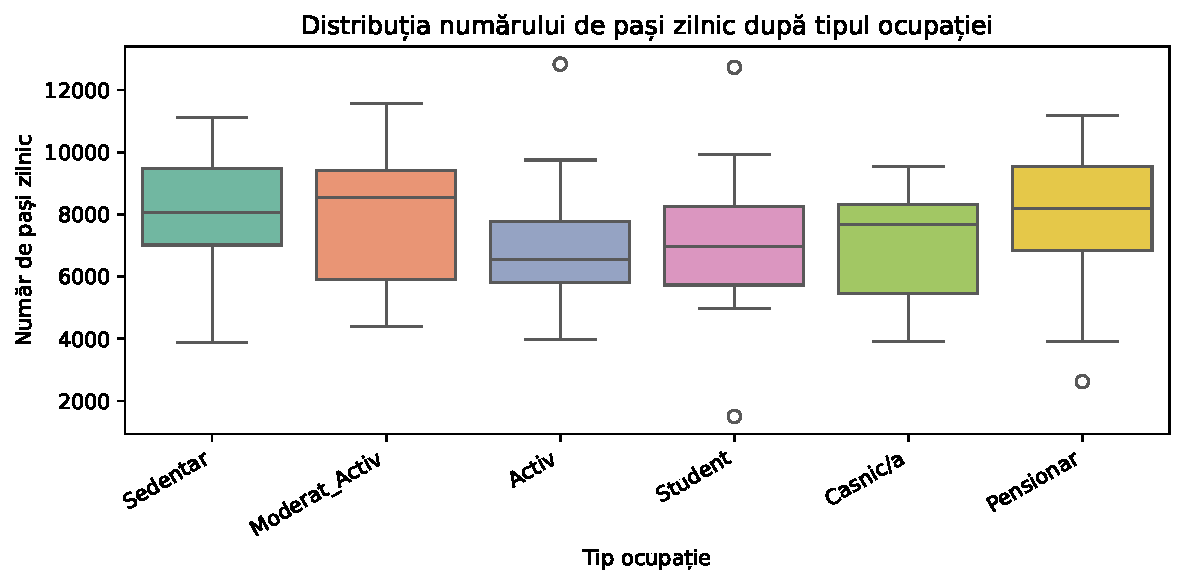
\includegraphics[width=0.8\textwidth]{../figuri/pasi_ocupatie_boxplot.pdf}
    \caption{Distribuția numărului de pași zilnic după tipul ocupației (boxplot)}
    \label{fig:pasi-ocupatie-box}
\end{figure}

În Figura~\ref{fig:pasi-ocupatie-bar} este prezentată și comparația mediilor numărului de pași zilnic pe tipuri de ocupație, împreună cu bare de eroare (deviația standard). Această reprezentare evidențiază faptul că anumite categorii, precum \textit{Sedentar} și \textit{Moderat\_Activ}, au niveluri medii de activitate fizică (măsurate prin numărul de pași) mai ridicate, în timp ce categoriile \textit{Activ} și \textit{Student} prezintă medii mai reduse, dar și o variabilitate relativ mare în interiorul grupului.

\begin{figure}[h!]
    \centering
    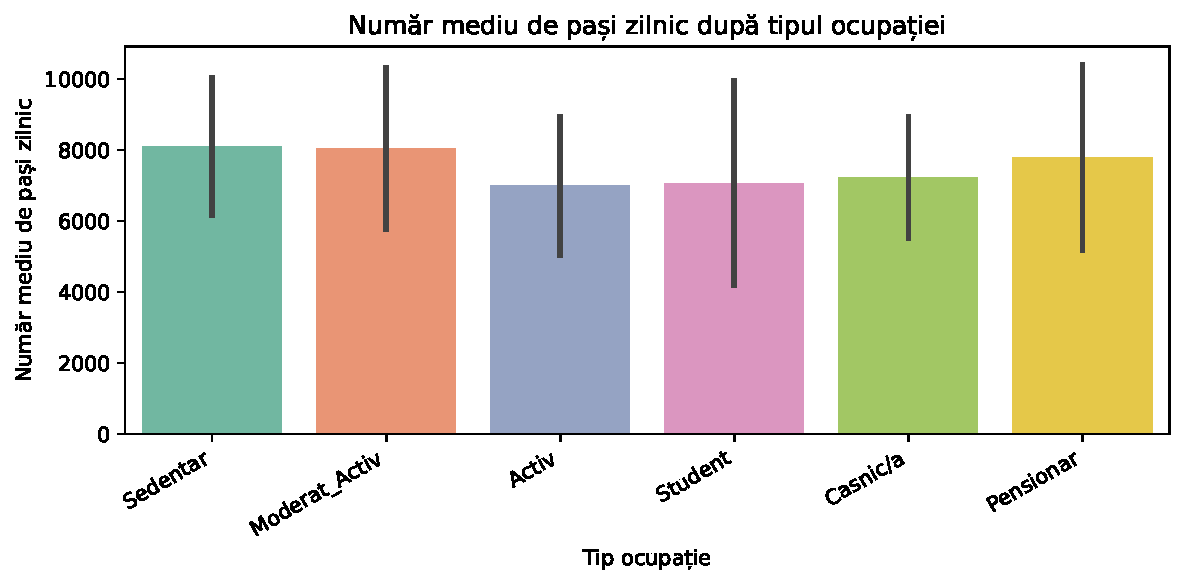
\includegraphics[width=0.8\textwidth]{../figuri/pasi_ocupatie_barplot.pdf}
    \caption{Număr mediu de pași zilnic după tipul ocupației cu bare de eroare (deviație standard)}
    \label{fig:pasi-ocupatie-bar}
\end{figure}

\pagebreak

% III. ANALIZA INDICATORILOR DE TENDINȚĂ CENTRALĂ ȘI DE VARIAȚIE
\section{Indicatori de tendință centrală și de variație}

\subsection{Indicatori pentru variabila \texorpdfstring{\texttt{Numar\_Pasi\_Zilnic}}{Numar\_Pasi\_Zilnic}}
% Prezinți formulele și valorile calculate (Python).

Pentru variabila principală analizată, \textit{Numar\_Pasi\_Zilnic}, calculăm principalii indicatori de poziție și variație: media aritmetică, varianța, abaterea standard și coeficientul de variație. Acești indicatori permit caracterizarea nivelului mediu al activității fizice zilnice (numărul de pași) și a gradului de dispersie a valorilor în jurul acestui nivel.

\subsubsection*{Media aritmetică}

Media aritmetică descrie nivelul mediu (tipic) al numărului de pași zilnic și este definită prin:

$$
\bar{x} = \frac{1}{n} \sum_{i=1}^{n} x_i,
$$

unde \(x_i\) reprezintă numărul de pași zilnic pentru observația \(i\), iar \(n\) este numărul total de observații. În cazul nostru, \(n = 100\), astfel că media numărului de pași zilnic este:

$$
\bar{x}_{\text{pasi}} = \frac{1}{100} \sum_{i=1}^{100} x_i \approx 7550{,}65 \text{ pași/zi}.
$$

Aceasta indică faptul că, în medie, persoanele din eșantion realizează aproximativ 7500–7600 de pași pe zi.

\subsubsection*{Varianța și abaterea standard}

Varianța eșantională măsoară dispersia valorilor în jurul mediei și este definită prin:

$$
s^2 = \frac{1}{n - 1} \sum_{i=1}^{n} (x_i - \bar{x})^2.
$$

Folosirea lui \(n-1\) la numitor (și nu \(n\)) corespunde varianței \emph{eșantionale}, care este un estimator nedeplasat al varianței populației. Pe baza datelor obținute, varianța numărului de pași zilnic este:

$$
s^2_{\text{pasi}} \approx 4\,756\,568{,}88 \ \text{pași}^2.
$$

Abaterea standard este rădăcina pătrată a varianței și exprimă dispersia în aceleași unități de măsură ca variabila analizată:

$$
s = \sqrt{s^2}.
$$

Pentru variabila \textit{Numar\_Pasi\_Zilnic}, abaterea standard este:

$$
s_{\text{pasi}} = \sqrt{4\,756\,568{,}88} \approx 2180{,}96 \text{ pași/zi}.
$$

Aceasta înseamnă că, în medie, numărul de pași zilnic al unei persoane se abate cu aproximativ 2100–2200 de pași față de media de \(7550{,}65\) pași.

\subsubsection*{Coeficientul de variație}

Pentru a evalua dispersia \emph{relativă} a valorilor față de medie (independent de unitățile de măsură), utilizăm coeficientul de variație:

$$
CV = \frac{s}{\bar{x}} \cdot 100\%.
$$

Aplicând formula pentru variabila \textit{Numar\_Pasi\_Zilnic}, obținem:

$$
CV_{\text{pasi}} = \frac{2180{,}96}{7550{,}65} \cdot 100\% \approx 28{,}88\%.
$$

Un coeficient de variație de aproximativ \(29\%\) indică un nivel \textit{moderat} al variabilității numărului de pași zilnic în cadrul eșantionului. Valorile nu sunt nici foarte concentrate în jurul mediei (cum ar fi cazul unui CV mic, sub \(15\%\)), dar nici extrem de dispersate (CV peste \(35\%\)). Aceasta sugerează o heterogenitate rezonabilă a nivelului de activitate fizică zilnică între persoanele investigate: există diferențe semnificative între indivizi, dar acestea nu sunt extreme la nivelul întregului eșantion.

\begin{table}[h!]
    \centering
    \caption{Rezumat al indicatorilor descriptivi pentru variabila \textit{Numar\_Pasi\_Zilnic}}
    \label{tab:rezumat-pasi}
    \begin{tabular}{l r p{7cm}}
        \hline
        \textbf{Indicator} & \textbf{Valoare} & \textbf{Interpretare} \\
        \hline
        Media aritmetică & 7550{,}65 pași/zi &
        Nivelul mediu (tipic) al numărului de pași zilnic. \\[2pt]
        Varianța & 4\,756\,568{,}88 pași\(^2\) &
        Măsoară dispersia valorilor în jurul mediei (mai greu de interpretat direct). \\[2pt]
        Abaterea standard & 2180{,}96 pași/zi &
        Abaterea medie a valorilor față de media numărului de pași. \\[2pt]
        Coeficientul de variație & 28{,}88\% &
        Dispersie relativă moderată a numărului de pași față de media sa. \\
        \hline
    \end{tabular}
\end{table}

% De introdus și mediană, quartile etc. + interpretare.

\subsection{Indicatori pe grupe}
% Ex: media și abaterea standard a numărului de pași pe sexe, pe tip ocupație etc.

Pe lângă analiza globală a variabilei \textit{Numar\_Pasi\_Zilnic}, este util să examinăm indicatorii de tendință centrală și de variație pe diferite subgrupe ale populației, pentru a surprinde eventuale diferențe structurale. În continuare, prezentăm media, abaterea standard și coeficientul de variație ale numărului de pași zilnic pe grupe de \textit{Sex}, \textit{Tip\_Localitate} și \textit{Tip\_Ocupatie}. Coeficientul de variație este calculat după formula:
$$
CV = \frac{s}{\bar{x}} \cdot 100\%,
$$
unde \(\bar{x}\) este media numărului de pași zilnic în cadrul grupei, iar \(s\) este abaterea standard corespunzătoare grupei.

\subsubsection*{Indicatori pe grupe de sex}

\begin{table}[h!]
    \centering
    \caption{Indicatori de variație pentru \textit{Numar\_Pasi\_Zilnic} pe grupe de sex}
    \label{tab:ind-grupe-sex}
    \begin{tabular}{l r r r}
        \hline
        \textbf{Sex} & \textbf{Medie (pași/zi)} & \textbf{Abatere standard (pași/zi)} & \textbf{CV (\%)} \\
        \hline
        Feminin  & 7448{,}11 & 2078{,}25 & 27{,}90 \\
        Masculin & 7641{,}58 & 2284{,}09 & 29{,}89 \\
        \hline
    \end{tabular}
\end{table}

Se observă că bărbații au, în medie, un număr ușor mai mare de pași zilnic decât femeile, însă coeficienții de variație sunt apropiați (aproximativ \(28\%\) pentru femei și \(30\%\) pentru bărbați), ceea ce indică un nivel similar al dispersiei relative în ambele grupe. Diferențele dintre sexe par să fie mai degrabă de nivel (poziție centrală) decât de variabilitate.

\subsubsection*{Indicatori pe grupe de tipul localității}

\begin{table}[h!]
    \centering
    \caption{Indicatori de variație pentru \textit{Numar\_Pasi\_Zilnic} pe grupe de tipul localității}
    \label{tab:ind-grupe-localitate}
    \begin{tabular}{l r r r}
        \hline
        \textbf{Tip localitate} & \textbf{Medie (pași/zi)} & \textbf{Abatere standard (pași/zi)} & \textbf{CV (\%)} \\
        \hline
        Rural & 7622{,}72 & 2106{,}38 & 27{,}63 \\
        Urban & 7496{,}28 & 2252{,}62 & 30{,}05 \\
        \hline
    \end{tabular}
\end{table}

Diferențele între mediul urban și cel rural sunt reduse atât din punct de vedere al mediilor, cât și al coeficienților de variație. Atât în mediul rural, cât și în mediul urban, coeficientul de variație se situează în jurul valorii de \(28\% - 30\%\), indicând o variabilitate relativ similară a numărului de pași zilnic. În acest eșantion, mediul de rezidență nu pare să fie asociat cu diferențe majore nici în nivelul mediu al activității fizice, nici în dispersia acesteia.

\subsubsection*{Indicatori pe grupe de tipul ocupației}

\begin{table}[h!]
    \centering
    \caption{Indicatori de variație pentru \textit{Numar\_Pasi\_Zilnic} pe grupe de tipul ocupației}
    \label{tab:ind-grupe-ocupatie}
    \begin{tabular}{l r r r}
        \hline
        \textbf{Tip ocupație} & \textbf{Medie (pași/zi)} & \textbf{Abatere standard (pași/zi)} & \textbf{CV (\%)} \\
        \hline
        Activ          & 6996{,}24 & 1943{,}66 & 27{,}78 \\
        Casnic/a       & 7222{,}62 & 1707{,}77 & 23{,}64 \\
        Moderat\_Activ & 8054{,}63 & 2274{,}84 & 28{,}24 \\
        Pensionar      & 7792{,}50 & 2605{,}47 & 33{,}44 \\
        Sedentar       & 8096{,}55 & 1930{,}32 & 23{,}84 \\
        Student        & 7071{,}45 & 2889{,}97 & 40{,}87 \\
        \hline
    \end{tabular}
\end{table}

În ceea ce privește tipul ocupației, se observă diferențe mai pronunțate atât în nivelul mediu al numărului de pași zilnic, cât și în variabilitatea relativă. Categoriile \textit{Sedentar} și \textit{Moderat\_Activ} prezintă cele mai ridicate medii ale numărului de pași (\(8096{,}55\), respectiv \(8054{,}63\) pași/zi), asociate cu coeficienți de variație în jurul valorii de \(24\% - 28\%\), ceea ce indică o dispersie moderată. Categoria \textit{Pensionar} are, de asemenea, o medie relativ ridicată (\(7792{,}50\) pași/zi), dar și un coeficient de variație mai mare (\(33{,}44\%\)), sugerând o heterogenitate mai pronunțată în cadrul acestui grup.

La polul opus, categoria \textit{Student} se remarcă printr-un nivel mediu relativ scăzut al numărului de pași (\(7071{,}45\) pași/zi), combinat cu cel mai ridicat coeficient de variație (\(40{,}87\%\)), ceea ce indică o variabilitate mare a comportamentelor de activitate fizică în rândul studenților. Grupurile \textit{Activ} și \textit{Casnic/a} prezintă medii mai scăzute (în jur de 7000–7200 pași/zi) și coeficienți de variație între aproximativ \(24\%\) și \(28\%\), corespunzători unei dispersii moderate.

În ansamblu, analiza pe grupe sugerează că tipul ocupației este asociat cu diferențe mai vizibile atât în nivelul mediu al activității fizice zilnice, cât și în variabilitatea acesteia, comparativ cu diferențele observate între sexe sau medii de rezidență.

% IV. ANALIZA UNEI SERII DINAMICE
\section{Analiza unei serii dinamice a numărului mediu de pași}

\subsection{Construirea seriei cronologice}
% Explici cum ai construit seria: de ex. media numărului de pași pe zi
% pentru o perioadă de 30 de zile: y_t, t = 1..30.

Pentru a analiza evoluția în timp a nivelului de activitate fizică zilnică, am construit o serie cronologică a numărului mediu de pași zilnic pe o perioadă de 24 de luni (ianuarie 2022 – decembrie 2023). Datele au fost generate sintetic pentru a ilustra metodologia de analiză a seriilor dinamice, incluzând o componentă de trend (tendință pe termen lung), o componentă sezonieră (variații ciclice legate de anotimpuri) și o componentă aleatoare (fluctuații neregulate).

Seria cronologică este prezentată în Tabelul~\ref{tab:serie-dinamica}, unde pentru fiecare lună este indicat numărul mediu de pași zilnic. Valorile variază între aproximativ 6400 și 8000 de pași pe zi, reflectând atât tendința generală de creștere, cât și variațiile sezoniere (de exemplu, valori mai ridicate în lunile de vară și mai scăzute în lunile de iarnă).

\begin{table}[h!]
    \centering
    \caption{Seria cronologică a numărului mediu de pași zilnic (2022–2023)}
    \label{tab:serie-dinamica}
    \begin{tabular}{l r | l r}
        \hline
        \textbf{Luna} & \textbf{Număr mediu pași/zi} & \textbf{Luna} & \textbf{Număr mediu pași/zi} \\
        \hline
        2022-01 & 6468{,}66 & 2023-01 & 7000{,}57 \\
        2022-02 & 6476{,}17 & 2023-02 & 7036{,}05 \\
        2022-03 & 6998{,}93 & 2023-03 & 7184{,}16 \\
        2022-04 & 7376{,}41 & 2023-04 & 7313{,}87 \\
        2022-05 & 7110{,}21 & 2023-05 & 7593{,}48 \\
        2022-06 & 7580{,}86 & 2023-06 & 7969{,}72 \\
        2022-07 & 7482{,}40 & 2023-07 & 8015{,}14 \\
        2022-08 & 7483{,}34 & 2023-08 & 7769{,}78 \\
        2022-09 & 7351{,}14 & 2023-09 & 7814{,}90 \\
        2022-10 & 7140{,}40 & 2023-10 & 7742{,}71 \\
        2022-11 & 7107{,}28 & 2023-11 & 7209{,}59 \\
        2022-12 & 6858{,}95 & 2023-12 & 7425{,}09 \\
        \hline
    \end{tabular}
\end{table}

Evoluția în timp a numărului mediu de pași zilnic este ilustrată grafic în Figura~\ref{fig:serie-dinamica}. Se poate observa o tendință generală de creștere pe parcursul celor doi ani, suprapusă peste o variație sezonieră: valorile tind să crească în lunile de primăvară și vară (martie–august) și să scadă în lunile de toamnă și iarnă (noiembrie–februarie). Această evoluție poate reflecta influența factorilor climatici și a obiceiurilor sezoniere asupra nivelului de activitate fizică.

\begin{figure}[h!]
    \centering
    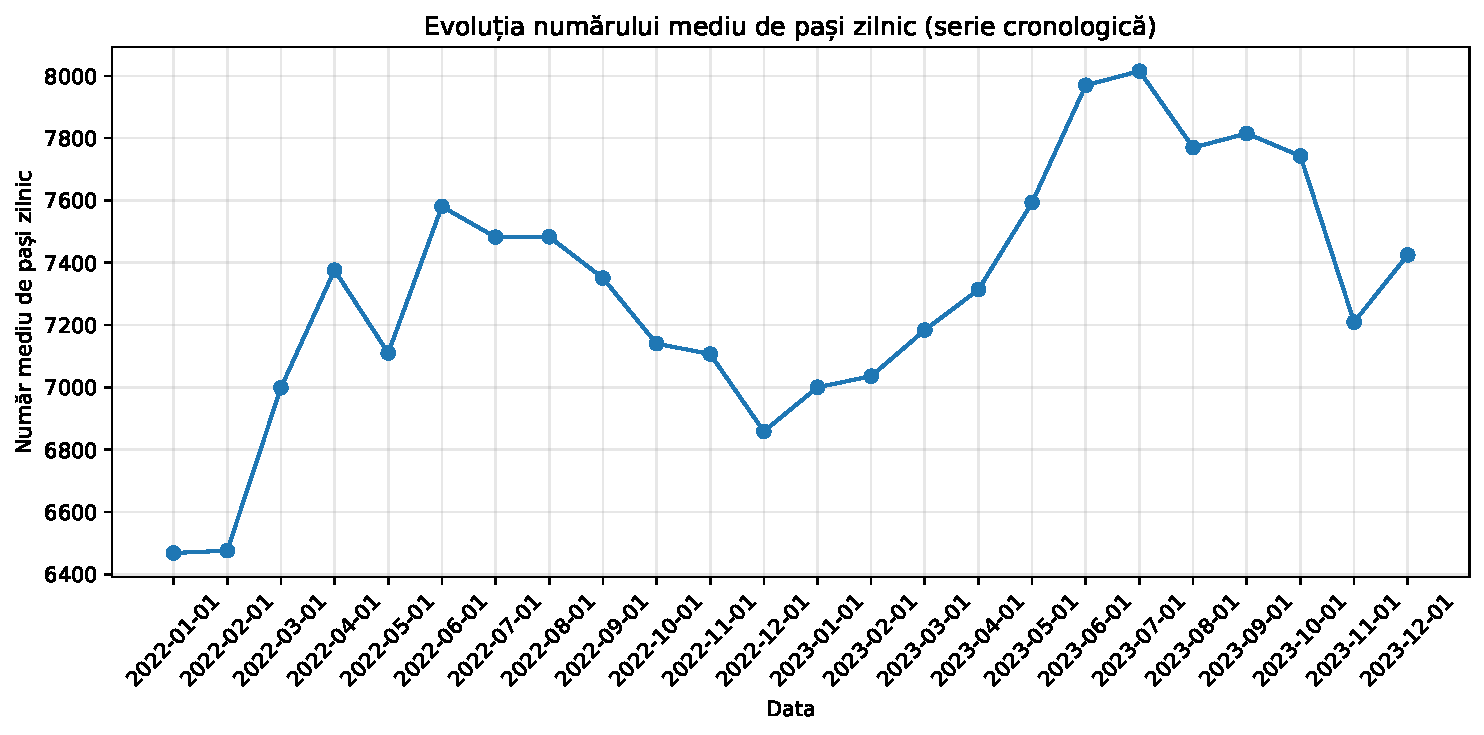
\includegraphics[width=0.9\textwidth]{../figuri/serie_dinamica_pasi.pdf}
    \caption{Evoluția numărului mediu de pași zilnic (serie cronologică, 2022–2023)}
    \label{fig:serie-dinamica}
\end{figure}


\subsection{Indicatori ai dinamicii}

Considerăm seria cronologică a numărului mediu de pași zilnic \(y_t\), pentru \(t = 1, 2, \dots, T\), unde fiecare \(y_t\) reprezintă numărul mediu de pași zilnic în luna \(t\). În cazul nostru, \(T = 24\) luni (ianuarie 2022 -- decembrie 2023).

\paragraph{Modificarea absolută (în lanț).}
Modificarea absolută în lanț măsoară diferența dintre nivelul seriei în două perioade consecutive:
\[
\Delta_{t/t-1} = y_t - y_{t-1}, \quad t = 2, \dots, T.
\]

\paragraph{Indicele (modificarea relativă în lanț).}
Indicele în lanț exprimă nivelul perioadei curente ca procent din nivelul perioadei precedente:
\[
I_{t/t-1} = \frac{y_t}{y_{t-1}} \cdot 100\%, \quad t = 2, \dots, T.
\]

\paragraph{Modificarea absolută şi indicele în bază fixă.}
Atunci când comparăm fiecare nivel al seriei cu nivelul iniţial \(y_1\), obţinem:
\[
\Delta_{t/1} = y_t - y_1, \quad
I_{t/1} = \frac{y_t}{y_1} \cdot 100\%, \quad t = 1, \dots, T.
\]

În Tabelul~\ref{tab:ind-dinamici} sunt prezentați indicatorii dinamici pentru o selecție de luni din perioada analizată (2022--2023).

\begin{table}[h!]
    \centering
    \caption{Indicatori ai dinamicii pentru numărul mediu de pași (selectiv)}
    \label{tab:ind-dinamici}
    \begin{tabular}{l r r r r r}
        \hline
        \textbf{Luna} &
        \(\mathbf{y_t}\) &
        \(\Delta_{t/t-1}\) &
        \(I_{t/t-1}\) (\%) &
        \(\Delta_{t/1}\) &
        \(I_{t/1}\) (\%) \\
        \hline
        2022-01 & 6468{,}66 &     --    &     --    &      0{,}00 & 100{,}00 \\
        2022-02 & 6476{,}17 &    7{,}51 & 100{,}12  &      7{,}51 & 100{,}12 \\
        2022-03 & 6998{,}93 &  522{,}76 & 108{,}07  &    530{,}27 & 108{,}20 \\
        2022-04 & 7376{,}41 &  377{,}48 & 105{,}39  &    907{,}75 & 114{,}03 \\
        2022-06 & 7580{,}86 &  470{,}65 & 106{,}62  &   1112{,}20 & 117{,}19 \\
        2022-12 & 6858{,}95 & -248{,}33 &  96{,}51  &    390{,}29 & 106{,}03 \\
        2023-01 & 7000{,}57 &  141{,}62 & 102{,}06  &    531{,}91 & 108{,}22 \\
        2023-06 & 7969{,}72 &  376{,}24 & 104{,}95  &   1501{,}06 & 123{,}21 \\
        2023-07 & 8015{,}14 &   45{,}42 & 100{,}57  &   1546{,}48 & 123{,}91 \\
        2023-11 & 7209{,}59 & -533{,}12 &  93{,}11  &    740{,}93 & 111{,}45 \\
        2023-12 & 7425{,}09 &  215{,}50 & 102{,}99  &    956{,}43 & 114{,}79 \\
        \hline
    \end{tabular}
\end{table}

Se observă că, de exemplu, între ianuarie 2022 şi martie 2022 nivelul mediu al numărului de paşi creşte de la \(6468{,}66\) paşi/zi la \(6998{,}93\) paşi/zi, ceea ce corespunde unei creşteri absolute în bază fixă de aproximativ \(530\) paşi/zi şi unui indice în bază fixă de circa \(108{,}20\%\). Cea mai mare valoare a seriei se înregistrează în iulie 2023 (\(8015{,}14\) paşi/zi), cu un indice în bază fixă de \(123{,}91\%\), ceea ce reprezintă o creştere de aproximativ \(24\%\) faţă de nivelul iniţial.

La finalul perioadei (decembrie 2023), nivelul seriei este cu aproximativ \(956\) paşi/zi mai mare decât în prima lună, ceea ce se traduce printr-un indice în bază fixă de aproximativ \(114{,}79\%\), adică o creştere globală de circa \(15\%\) faţă de nivelul iniţial. Modificările în lanț evidenţiază fluctuaţii lunare semnificative, de exemplu o scădere bruscă de \(533\) paşi între octombrie şi noiembrie 2023 (indice în lanţ de \(93{,}11\%\)), urmată de o revenire în decembrie 2023.

\begin{figure}[h!]
    \centering
    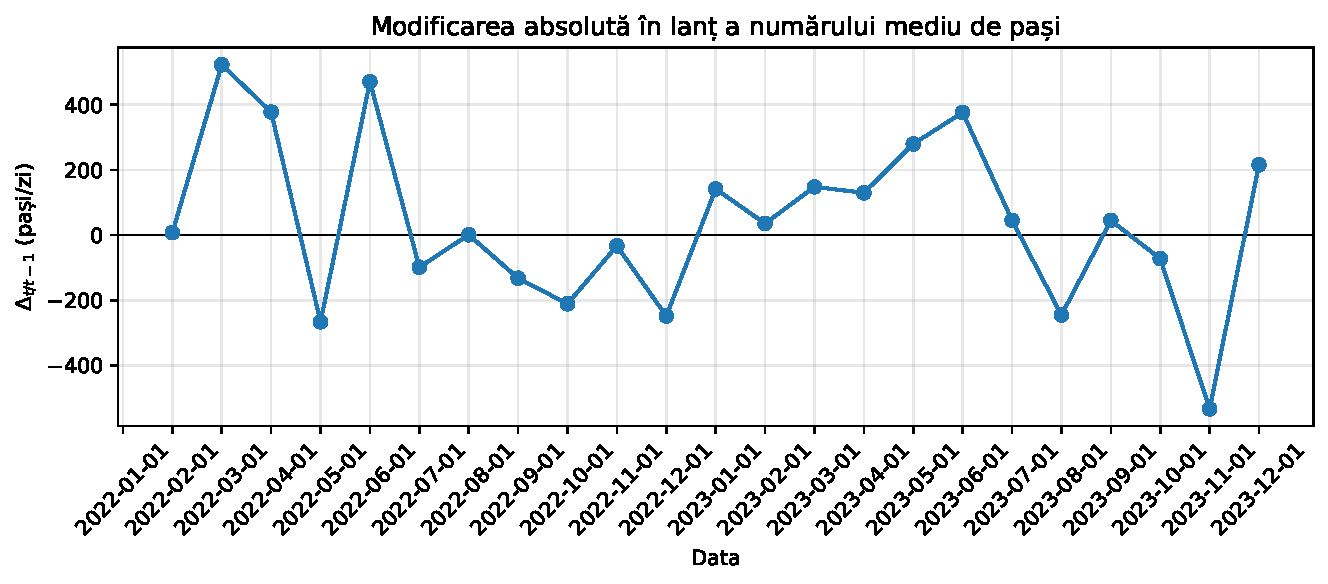
\includegraphics[width=0.9\textwidth]{../figuri/delta_lant_pasi.pdf}
    \caption{Modificarea absolută în lanț a numărului mediu de pași zilnic}
    \label{fig:delta-lant-pasi}
\end{figure}

Modificarea absolută în lanț \(\Delta_{t/t-1}\) evidențiază variațiile de la o lună la alta ale numărului mediu de pași. Valorile pozitive indică luni în care activitatea fizică medie a crescut față de luna precedentă, în timp ce valorile negative marchează scăderi. Se observă alternanța perioadelor de creștere (de exemplu, martie--aprilie 2022 sau mai--iulie 2023) cu perioade de scădere (de exemplu, noiembrie 2023), ceea ce reflectă atât efecte sezoniere, cât și fluctuații aleatoare.

\begin{figure}[h!]
    \centering
    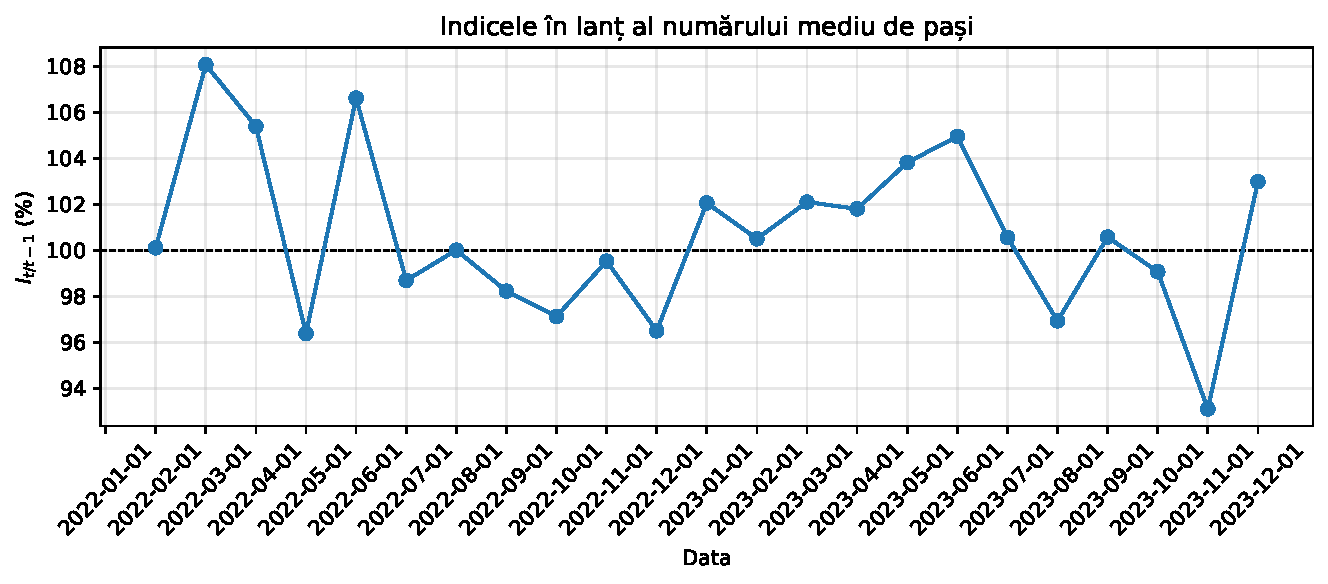
\includegraphics[width=0.9\textwidth]{../figuri/indice_lant_pasi.pdf}
    \caption{Indicele în lanț al numărului mediu de pași zilnic}
    \label{fig:indice-lant-pasi}
\end{figure}


Indicele în lanț \(I_{t/t-1}\) exprimă nivelul perioadei curente ca procent din nivelul perioadei precedente. Valori peste \(100\%\) indică o creștere a numărului mediu de pași, iar valori sub \(100\%\) indică o scădere. În majoritatea lunilor, indicele se situează relativ aproape de \(100\%\), ceea ce sugerează variații lunare moderate, cu excepția unor luni în care se înregistrează scăderi mai accentuate (de exemplu, noiembrie 2023, cu un indice de aproximativ \(93\%\)).

\begin{figure}[h!]
    \centering
    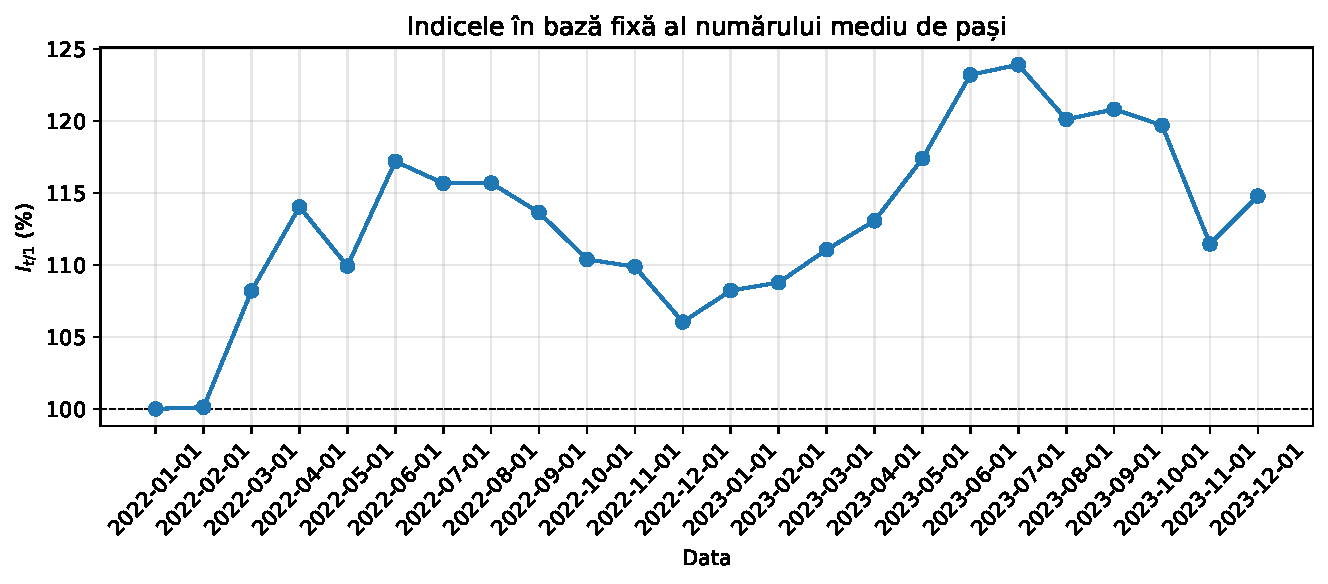
\includegraphics[width=0.9\textwidth]{../figuri/indice_baza_pasi.pdf}
    \caption{Indicele în bază fixă al numărului mediu de pași zilnic}
    \label{fig:indice-baza-pasi}
\end{figure}

Indicele în bază fixă \(I_{t/1}\) compară fiecare lună cu luna inițială (ianuarie 2022). Se observă o tendință generală de creștere: în special în a doua parte a perioadei, indicele depășește frecvent \(115\%\), ceea ce indică o creștere cumulată importantă a nivelului mediu de activitate fizică față de începutul intervalului analizat.

\pagebreak

\subsection{Indicatori medii ai seriei}

\subsection{Indicatori medii ai seriei}

Pentru caracterizarea globală a evoluției numărului mediu de pași zilnic pe întreaga perioadă analizată (24 de luni), utilizăm următorii indicatori medii: media nivelurilor seriei, modificarea medie absolută şi rata medie a creşterii. Calculul numeric al acestor indicatori a fost realizat în Python, pe baza valorilor lunare prezentate anterior.

\paragraph{Media seriei.}
Media nivelurilor seriei se calculează ca medie aritmetică a valorilor lunare:
\[
\bar{y} = \frac{1}{T} \sum_{t=1}^{T} y_t,
\]
unde \(T\) este numărul total de perioade (luni), iar \(y_t\) este numărul mediu de pași zilnic în luna \(t\). Pentru seria analizată (\(T = 24\)), obţinem:
\[
\bar{y} = \frac{1}{24} \sum_{t=1}^{24} y_t \approx 7312{,}91 \text{ pași/zi}.
\]
Aceasta înseamnă că, în medie, pe întreaga perioadă 2022--2023, nivelul activității fizice a fost de aproximativ 7300 de pași pe zi.

\paragraph{Modificarea medie absolută.}
Modificarea medie absolută măsoară, în medie, cu câți pași pe zi se modifică nivelul seriei de la o lună la alta şi se calculează astfel:
\[
\overline{\Delta} = \frac{y_T - y_1}{T-1},
\]
unde \(y_1\) este nivelul din prima lună, iar \(y_T\) nivelul din ultima lună. Pentru datele noastre:
\[
y_1 = 6468{,}66, \quad y_{24} = 7425{,}09, \quad T = 24,
\]
de unde rezultă:
\[
\overline{\Delta} = \frac{7425{,}09 - 6468{,}66}{24 - 1}
= \frac{956{,}43}{23} \approx 41{,}58 \text{ pași/zi/lună}.
\]
Astfel, pe ansamblul perioadei, numărul mediu de pași zilnic a crescut, în medie, cu aproximativ 40–45 de pași pe zi de la o lună la alta.

\paragraph{Rata medie a creșterii.}
Rata medie a creșterii exprimă, în termeni relativi (procente), creșterea medie lunară a seriei, fiind definită prin:
\[
\overline{i} = \sqrt[T-1]{\frac{y_T}{y_1}} - 1,
\]
adică rata constantă \( \overline{i} \) care, aplicată succesiv în fiecare lună, ar conduce de la nivelul inițial \(y_1\) la nivelul final \(y_T\).

Înlocuind valorile seriei:
\[
\overline{i} = \sqrt[23]{\frac{7425{,}09}{6468{,}66}} - 1
= \sqrt[23]{1{,}1479} - 1 \approx 0{,}0060,
\]
adică:
\[
\overline{i} \cdot 100\% \approx 0{,}60\% \text{ pe lună}.
\]

Aceasta înseamnă că, în medie, numărul mediu de pași zilnic a înregistrat o creștere relativă de aproximativ \(0{,}6\%\) pe lună pe întreaga perioadă analizată. Deși creșterile lunare efective pot fi uneori mai mari sau chiar negative (scăderi), rata medie de creștere surprinde tendința globală de creștere moderată a nivelului de activitate fizică zilnică.

\paragraph{Rezumat numeric.}
În Tabelul~\ref{tab:rezumat-ind-medii-serie} sintetizăm cei trei indicatori medii calculați pentru seria cronologică a numărului mediu de pași zilnic.

\begin{table}[h!]
    \centering
    \caption{Rezumat al indicatorilor medii ai seriei cronologice}
    \label{tab:rezumat-ind-medii-serie}
    \begin{tabular}{l r p{7cm}}
        \hline
        \textbf{Indicator} & \textbf{Valoare} & \textbf{Interpretare} \\
        \hline
        Media seriei \(\bar{y}\) &
        7312{,}91 pași/zi &
        Nivelul mediu, pe întreaga perioadă 2022--2023, al numărului de pași zilnic. \\[2pt]
        
        Modificarea medie absolută \(\overline{\Delta}\) &
        41{,}58 pași/zi/lună &
        Creșterea medie, în unități absolute, a numărului mediu de pași de la o lună la alta. \\[2pt]
        
        Rata medie a creșterii \(\overline{i}\) &
        0{,}60\% pe lună &
        Creșterea medie relativă lunară a nivelului seriei; indică o tendință globală de creștere moderată. \\ 
        \hline
    \end{tabular}
\end{table}

% CONCLUZII
\chapter*{Concluzii}
\addcontentsline{toc}{chapter}{Concluzii}

Prezentul proiect a avut ca scop realizarea unei analize statistice a nivelului de activitate fizică zilnică (măsurat prin numărul de pași) în funcție de caracteristicile demografice și de stil de viață, utilizând un set de date sintetice. Analiza a parcurs etapele specifice unei observații statistice, de la sistematizarea și prezentarea datelor, până la calculul indicatorilor de tendință centrală și de variație, și analiza unei serii dinamice.

\subsection*{Principalele descoperiri}

\begin{itemize}
    \item \textbf{Distribuția generală a numărului de pași:} Variabila \textit{Numar\_Pasi\_Zilnic} a prezentat o medie de aproximativ \(7550{,}65\) pași/zi, cu o abatere standard de \(2180{,}96\) pași/zi și un coeficient de variație de \(28{,}88\%\). Aceasta indică un nivel mediu de activitate fizică și o dispersie moderată a valorilor în cadrul eșantionului.
    
    \item \textbf{Diferențe pe grupe demografice:}
    \begin{itemize}
        \item \textit{Sex:} Bărbații au înregistrat un număr mediu de pași ușor mai mare decât femeile (7641{,}58 vs. 7448{,}11 pași/zi), însă cu o variabilitate relativ similară.
        \item \textit{Tip\_Localitate:} Diferențele între mediul urban și rural au fost minime, atât în ceea ce privește media, cât și variabilitatea numărului de pași.
        \item \textit{Tip\_Ocupatie:} Această variabilă a relevat diferențe mai pronunțate. Categoriile \textit{Sedentar} și \textit{Moderat\_Activ} au avut cele mai ridicate medii ale numărului de pași, în timp ce \textit{Student} a prezentat cea mai mare variabilitate (CV de \(40{,}87\%\)) și o medie relativ scăzută. Aceasta sugerează că ocupația este un factor mai influent în determinarea nivelului și variabilității activității fizice.
    \end{itemize}
    
    \item \textbf{Analiza seriei dinamice:}
    \begin{itemize}
        \item Seria cronologică a numărului mediu de pași zilnic pe 24 de luni a evidențiat o tendință generală de creștere, suprapusă peste o componentă sezonieră (valori mai mari vara, mai mici iarna).
        \item Indicatorii medii ai seriei au confirmat o creștere medie de \(41{,}58\) pași/zi/lună și o rată medie de creștere de \(0{,}60\%\) pe lună, indicând o evoluție pozitivă, dar moderată, a activității fizice pe parcursul celor doi ani.
        \item Analiza modificărilor absolute și a indicilor a relevat fluctuații lunare semnificative, influențate de sezonalitate, dar și o creștere cumulată de aproximativ \(15\%\) a numărului mediu de pași de la începutul până la sfârșitul perioadei analizate.
    \end{itemize}
\end{itemize}

\subsection*{Implicații și direcții viitoare}

Rezultatele sugerează că, deși există o tendință generală de creștere a activității fizice, factori precum ocupația pot influența semnificativ comportamentul individual. Pentru studenți, de exemplu, variabilitatea mare și media relativ scăzută ar putea indica necesitatea unor intervenții specifice pentru promovarea unui stil de viață mai activ.

Pe viitor, analiza ar putea fi extinsă prin:
\begin{itemize}
    \item Includerea unui volum mai mare de date și a unei perioade mai lungi pentru seria cronologică, pentru o estimare mai robustă a trendului și sezonalității.
    \item Aplicarea unor metode de descompunere a seriilor cronologice (e.g., STL, X-13 ARIMA-SEATS) pentru o separare mai clară a componentelor de trend, sezon și reziduală.
    \item Realizarea unei analize de regresie multiple pentru a identifica factorii demografici și de stil de viață care influențează cel mai puternic numărul de pași zilnic.
    \item Utilizarea unor teste de ipoteză pentru a valida statistic diferențele observate între grupe.
\end{itemize}

Acest proiect oferă o bază solidă pentru înțelegerea statistică a activității fizice, deschizând calea către studii mai aprofundate și intervenții țintite pentru îmbunătățirea sănătății publice.

\end{document}